\chapter{Estado de la Cuestión}
\label{cap:estadoDeLaCuestion}

En este capítulo, se estudiarán detalladamente las simulaciones basadas en agentes de inteligencia artificial y modelos de lenguaje, así como las complejidades en las relaciones sociales y la interacción persona-ordenador. El objetivo fundamental es contextualizar la evolución histórica y actual de estos temas, destacando la relevancia de su estudio y desarrollo, subrayando la importancia de que estos sistemas puedan ser fácilmente extensibles y utilizados por profesionales de distintos ámbitos. El capítulo se dividirá en varios puntos, los cuales se pueden englobar en dos secciones.

La primera sección del estado de la cuestión se centra en las simulaciones basadas en agentes y su aplicación en entornos de inteligencia artificial. Se explorarán los avances tecnológicos, las metodologías y los desarrollos más recientes que han influido en la creación de sistemas de simulación avanzados. Asimismo, se examinará la relación de estos agentes con modelos de lenguaje, identificando los desafíos de esta convergencia tecnológica.

Después, se revisarán los desarrollos más destacados en procesamiento del lenguaje natural (PLN) y cómo estos contribuyen a la mejora de la interacción entre humanos y sistemas de inteligencia artificial. Además, se explorarán los aspectos psicológicos relacionados con las relaciones sociales en el contexto de la informática. También se centrará en la interacción persona-ordenador, se analizarán las tendencias actuales en diseño centrado en el usuario y las estrategias para garantizar que las simulaciones de inteligencia artificial sean accesibles a todos los públicos, independientemente de su desconocimiento sobre la tecnología.
\section{Agentes}

Los sistemas informáticos se asumen como obedientes máquinas que siguen todas las instrucciones que les solicitamos o programamos, resultando en un fallo del sistema o pérdida de archivos en el mejor de los casos o en la pérdida de vidas en el peor. Sin embargo hay ciertas aplicaciones o tareas en las que necesitamos una capacidad de resiliencia y decisión que con los sistemas tradicionales no es posible obtener. Sobre todo en entornos de rápido cambio, impredecibles y donde la cantidad de posibles situaciones no permita la posibilidad de plantearse cualquier escenario desde el diseño.

Un típico ejemplo de la necesidad de este tipo de sistemas es el envío de una sonda espacial a una distancia de la tierra que imposibilite el uso de un equipo humano que realice el seguimiento y toma de decisiones ante cualquier eventualidad imprevista, debido al retardo en la comunicación con la sonda debido a la distancia. Estas necesidades llevan a empresas como la NASA a investigar en agentes con más capacidad de autonomía para tener un mejor desempeño y confianza en este tipo de sistemas\footnote{\url{https://s3vi.ndc.nasa.gov/ssri-kb/static/resources/WS02-03-010.pdf}}.

Otro ejemplo, en una situación más cercana, sería la forma en que se localizan, actualizan y registran las páginas web en Internet. Cualquiera que se haya visto envuelto en el desarrollo de una página web probablemente se haya topado con un archivo llamado robots.txt, que es la forma que tienes de comunicarte con los agentes que Google utiliza para registrar o actualizar las páginas a través de Internet\footnote{\url{https://developers.google.com/search/docs/crawling-indexing/robots/intro?hl=es}}.

A pesar de que \textit{Agente} es un término ampliamente usado en la literatura y los sistemas con los que interactuámos cada día, no hay un consenso en la definición de Agente, el mayor acuerdo que se encuentra en torno a esta definición es la centralidad que ocupa la autonomía para un Agente. Parte del desacuerdo en esta definición se debe al amplio número de sectores en los que es utilizado, teniendo cada uno de estos unas necesidades muy distintas, siendo necesaria alguna característica de los Agentes en ciertos sectores pero totalmente indeseables en otros, un ejemplo sería la capacidad de aprender de los Agentes. En cualquier caso se puede tomar prestada la definición dada en \cite{weiss1999multiagent} para tener una idea más cercana de lo que pretendemos expresar al hablar de Agentes.

\[Un Agente es un \textit{sistema computacional} que se encuentra en cierto \textit{entorno}, y es capáz de \textit{actuar} de forma autónoma en este entorno con el fin de cumplir sus objetivos de diseño\]

%Breve descripción
\subsection{Principios en el diseño}

Entre los factores más importantes a la hora de diseñar un Agente se encuentran los siguiente:

\begin{itemize}
	\item\textbf{La capacidad de control del Entorno} En el mejor de los casos el Agente tiene un control parcial sobre el entorno, pero no en la mayoría.
	\item\textbf{Decisión de la acción a ejecutar} Esta toma de decisiones se puede ver afectada por el tipo de entorno en el que nos encontramos y siempre está enfocada en conseguir los objetivos definidos de la forma más satisfactoria posible.
	\item\textbf{No-determinismo de las acciones ejecutadas} La falta de control supone que una misma acción no dará siempre los mismos resultados.
	\item\textbf{Posibilidad de fallo} El mencionado no-determinismo nos lleva, en numerosas ocasiones, a no obtener el resultado deseado, por ello, incluso en los Agentes más sencillos, hay que tener en cuenta la posibilidad de fallo.
\end{itemize}

Con lo dicho hasta el momento damos cabida a un gran número de sistemas, en esta definición cabe cualquier \textit{daemon} de nuestro sistema, por ejemplo el programa \textbf{xbiff} que es capaz de monitorear un sistema UNIX y notificar al usuario en caso de que haya un nuevo correo.

\subsection{Agentes inteligentes}

Una aplicación más buscada y útil son los Agentes Inteligentes, la diferencia con los anteriores es la flexibilidad que estos tienen de actuar de forma autónoma y flexible para cumplir con sus objetivos de diseño. Por flexible entendemos lo descrito en \cite{jennings1998agent}:

\begin{itemize}
	\item\textbf{Sensible a su entorno} siendo capaces de reaccionar en los momentos oportunos en los que su entorno cambia.
	\item\textbf{Proactivo} además de ser capaces de responder a los cambios deben ser capaces de tomar la iniciativa en la búsqueda de cumplir sus objetivos.
	\item\textbf{Sociable} también han de ser capaces de comunicarse con otros agentes o humanos, cuando lo consideren necesario, para cumplimentar sus objetivos.
\end{itemize}

Este tipo de sistemas permite encarar un gran número de problemas y desarrollar sistemas en los que podemos disponer de Agentes Inteligentes capaces de realizar nuevas tareas. Un claro ejemplo de esto, que ya mencionábamos anteriormente, es Internet, donde tenemos una gran red de organizaciones desplegando información y cada una de ellas siguiendo sus propios objetivos y metodologías, haciendo de este un entorno muy heterogéneo y dinámico.

Este tipo de agentes es también un componente central en \cite{park2023generative}, siendo en base a estos y su interacción (entre ellos y su entorno), que obtenemos las complicadas dinámicas que acabamos observando. Viendo una vez más de la capacidad de estos sistemas para acomodarse en dominios cambiantes y de gran complejidad.

\section{Simulaciones basadas en agentes}

En este apartado mostraremos de forma superficial el concepto de Simulaciones basadas en Agentes, así como numerosos ejemplos en los que se ha visto aplicada esta técnica, ya que es un concepto central a la hora de desarrollar el trabajo \cite{park2023generative} en el que se basa nuestro TFG.
Las Simulaciones basadas en Agentes, o también conocidas como Agent-Based Model (ABM), tratan de dar lugar a sistemas complejos a través del uso de agentes. En base a la interacción, entre agentes y el entorno, se pretende generar comportamientos y patrones a nivel de sistema.
Este tipo de sistemas se caracteriza por:
\begin{itemize}
	\item Tener un conjunto de agentes que siguen reglas sencillas
	\item Estos agentes interactúan entre sí de forma continuada
	\item Hay características a nivel de sistema que ocurren de forma emergente
	\item Las reglas elegidas para los agentes se entienden como fundamentales
	\item Una vez establecidas dichas reglas se observa la evolución del sistema (aquí es donde frecuentemente ocurre el fenómeno de la emergencia)
	\item El dominio de los fenómenos que se pretende recrear son de gran complejidad
\end{itemize}

Es por esta última característica que la variedad de escenarios o fenómenos recreables se vuelve tan amplio. Permitiendo a una gran cantidad de disciplinas hacer uso de estas técnicas. Tenemos ejemplos en multitud de Ciencias Sociales, Organizacionales, Ecológicas, Económicas, etc...
Unido a esto, tenemos la importancia que se ha conferido al entendimiento de un alto número de sistemas complejos en múltiples ámbitos del conocimiento, por ejemplo tenemos el clima terrestre, la ecología, el cerebro, las relaciones sociales, etc...
Así se junta una técnica muy versátil con un necesidad, ampliamente extendida, de recrear y analizar sistemas de alta complejidad, los cuales escapan a los clásicos modelos lineales o analíticos.

\subsection{Historia de las Simulaciones basadas en agentes}

Entre las décadas de los 50 y los 70, trabajos como la máquina auto-replicante \citep{neumann1966theory} , de Von Neumann, o como el Juego de la Vida \citep{gardner1970fantastic}, de John Conway, dieron cabida y avance al concepto de Autómata celular, siendo esta una de las primeras formas de Simulación basada en agentes.

Poco tiempo después vemos varios modelos que empleaban Simulaciones basadas en agentes para estudiar diversidad de fenómenos. Tenemos ejemplos en la política \citep{schelling1971dynamic}, la Teoría de Juegos (mediante un torneo organizado por Robert Axelrod para evaluar distintas estrategias del Dilema del Prisionero), o la ecología \citep{hogeweg1983ontogeny}.

En los 90 surge una expansión notable en el interés por estas técnicas. Esto se ve reflejado en diversos trabajos, de notable envergadura, llevados a cabo por varias universidades e investigadores provenientes de multitud de disciplinas, como ejemplos tenemos \cite{epstein1996growing} de Sugarscape, \textit{Computational Analysis of Social and Organizational Systems} (CASOS)\footnote{\url{http://www.casos.cs.cmu.edu/}} de la Carnegie Mellon University, o \cite{kohler2000dynamics} del Santa Fe Institute  entre otros.

También surgieron revistas enfocadas a las sociedades virtuales y sus simulaciones, como la Journal of Artificial Societies and Social Simulations (JASSS) o la Complex Adaptive Systems Modeling (CASM) de Springer.

La efectividad de estos métodos acabó saltando fuera del ámbito de la investigación y encontrando un hueco en la sociedad. Lo podemos ver reflejado en el surgimiento de varias organizaciones, durante la misma década, centradas en el estudio y exploración de Simulaciones sociales y técnicas de organización efectiva -NAACSOS\footnote{\url{http://www.casos.cs.cmu.edu/naacsos/index.php}}, ESSA\footnote{\url{http://www.essa.eu.org/}}, PAAAESSA\footnote{\url{http://www.paaa.asia/\#:~:text=Pacific\%2DAsian\%20Association\%20for\%20Agent,European\%20Social\%20Simulation\%20Association\%2C\%20ESSA}}- a través de Simulaciones basadas en Agentes.

Con esta breve revisión queda claro el amplio rango de aplicación de estos modelos, además del gran interés que suscitan por la misma razón.

\subsection{Principios de las Simulaciones basadas en agentes}

Las simulaciones basadas en agentes se basan principalmente en el modelo computacional de los Sistemas Multiagente. Este tipo de sistemas forman un nuevo paradigma de computación enfocado en resolver tareas que serían imposibles de resolver para un sistema centralizado, bien por la complejidad de diseñar e implementar soluciones centralizadas, o bien por el pobre rendimiento que estas obtendrían.

Aparte de la naturaleza descentralizada del problema, se encuentra el otro componente central en este paradigma, los agentes. En este tipo de sistemas son los Agentes y las interacciones que hay entre ellos y su entorno los que dan lugar a las dinámicas que hacen de es interés este paradigma.

Es en la conjunción de estos dos conceptos donde se desvelan los elementos centrales de un Sistema multiagente, estos son, los Protocolos de comunicación entre Agentes, los protocolos de interacción entre Agentes y Entorno y el Entorno.

Estas características se van a explicar basandonos en \cite{weiss1999multiagent}

\subsubsection{El entorno}

El entorno se puede pensar como la infraestructura que especifica los distintos protocolos de comunicación e interacción entre agentes y entorno. Permitiendo siempre la interacción, en mayor o menor medida, de los Agentes con "lo que les rodea". Otros aspectos clave en el diseño del entorno son la falta de centralización del entorno y que estos están poblados por Agentes. 

Además de esas consideraciones están otras que surgen a la hora de diseñarlo, teniendo en cuenta que estas especificaciones engloban cualquier tipo de sistema multiagente.

\begin{itemize}
	\item\textbf{Infraestructura de comunicación} En la que se tiene en cuenta el tipo de comunicaciones que se puede dar entre los agentes, dando la posibilidad de que esta sea Broadcast o Unicast, Memoria compartida o mensajes a través de la red, comunicación sincrona o asíncrona, etc...
	\item\textbf{Protocolos de mensaje} Si la comunicación se dá entre agentes en distintas redes abrá que considerar el tipo de protocolos de red que utilizarán para la comunicación (HTTP, HTML...).
	\item\textbf{Servicios de seguridad} Para garantizar una participación de agentes legítimos en el sistema.
	\item\textbf{Soporte de operaciones} Que garantice una consistencia en las interacciones que se dén en el sistema.
\end{itemize}

Además de estas características propias del entorno, están las relativas al entorno-agente:

\begin{itemize}
	\item\textbf{Percepción del entorno} Cuánto sabe el agente sobre el entorno.
	\item\textbf{Predecible} Cómo de predecible es el entorno para el agente.
	\item\textbf{Controlable} Cuán modificable es el entorno por el agente.
	\item\textbf{Dependiente del pasado} Cuánta dependencia tienen los futuros estados del sistema de los estados previos.
	\item\textbf{Naturaleza Teleológica de las partes} Qué capacidad de acción tienen las otras partes del sistema desde el punto de vista del agente.
	\item\textbf{A tiempo real} El entorno es cambiante durante el proceso de toma de decisión del agente.
\end{itemize}

\subsubsection{Protocolos de comunicación entre agentes}

Los agentes capaces de realizar esta acción son entes activos, capaces de percibir, razonar y actuar. Entre las acciones disponibles de un agente asumimos que se encuentra la de comunicarse con otros agentes, aunque también tiene su parte de percepción (al ser capaz de recibir mensajes de otros agentes para que exista una verdadera comunicación).

El objetivo de la comunicación entre Agentes es conseguir mejores resultados para ellos o para el sistema/sociedad de agentes (según si el Agente es cooperativo o no). Un resultado favorable de que haya comunicación entre Agentes es que da la posibilidad de que haya coordinación en el comportamiento y sus acciones, dando lugar a sistemas más coherentes. Esta coherencia se puede interpretar como la capacidad del sistema de actuar como una unidad, lograr esto a través de Agentes independientes es algo difícil de lograr sin ningún tipo de comportamiento centralizado. 

A la hora de tratar de establecer la forma de comunicación entre Agentes surgen complicaciones a las que prestar atención, como pueden ser las siguientes:

\begin{itemize}
	\item\textbf{Mensaje Descriptivo vs Prescriptivo} Habiendo una diferencia entre mensajes que describen hechos y mensajes que describen acciones o comportamientos, siendo el primero de estos igual de esencial que el segundo, pero menos adoptado por la dificultad que tiene hacer que una Agente sea capaz de emitir dichos mensajes.
	\item\textbf{Significado Personal vs Convencional} También se ha de tener en cuenta la diferencia de significado de un mensjae que puede haber entre el que lo emite y quien lo recibe.
	\item\textbf{Contexto} Igual de importante que el contenido de un mensaje e ssu contexto. Debiendo tener en cuenta el estado del agente receptor y el del entorno.
	\item\textbf{Alcance del lenguaje} Compromiso entre expresividad del lenguaje y complejidad a la hora de manejarlo.
	\item\textbf{Identidad} Se podría considerar parte del \textbf{Contexto} del lenguaje, tiene en cuenta los roles y partes involucradas en el mensaje.
\end{itemize}

Otros factores a tener en cuenta a la hora de especificar los protocolos de comunicación entre Agentes son el tipo de mensajes (dependiente del tipo de Agente emisor), los niveles de comunicación, intención de la comunicación, etc... 

No los veremos en detalle debido a la extensión del campo y a que en el sistema multiagente relativo al trabajo en que nos basamos (\cite{park2023generative}) los protocolos de comunicación están englobados dentro de la arquitectura de Agente propuesta. Además de que varios de los puntos a tener en cuenta son relegados a la hora de adoptar las respuestas del LLM subyacente como los directores de acción de los Agentes.

\subsubsection{Protocolos de interacción entre agentes}

Los protocolos de interacción se encargan de llevar a cabo el intercambio de una serie de mensajes entre Agentes -Una conversación-. Se puede hacer una distinción entre los tipos de protocolos en base a si los Agentes actúan por objetivos individuales o comunes. En el caso de los objetivos individuales lo único que se pretende con los protocolos de interacción es maximizar las "ganancias". Al contrario, al haber Agentes con objetivos comunes, los protocolos de interacción tratan de lograr una coherencia global sin afectar a la autonomía de los Agentes y sin un control global explícito. Para lograr esto se tienen en cuenta varios aspectos como determinar objetivos o tareas comunes, evitar conflictos innecesarios o reunir conocimiento y pruebas.

\subsection{Uso reciente de Simulaciones basadas en agentes}

Como ya hemos visto en el apartado anterior, el rango de aplicaciones que este tipo de métodos tiene es amplio. En este apartado mencionaremos, superficialmente, avances significativos en distintos campos, a través del uso de esta técnica. Nos centraremos en los campos más relacionados al trabajo en el que nos basamos en este documento \cite{park2023generative}.

\begin{itemize}
	\item \textbf{Estudios  de Marketing} En este ámbito tenemos como ejemplo \cite{rand2011agent}, el cual propone líneas generales de desarrollo de Simulaciones basadas en Agentes que cumplan con ciertos estándares ámpliamente aceptados en ese ámbito en concreto, cumpliendo con la necesidad de establecer una forma común de proceder al hacer uso de las Simulaciones basadas en Agentes.

Así vemos, con este trabajo, que en el ámbito del marketing ya se ha buscado la aplicación de este tipo de técnicas.
	\item \textbf{Psicología Organizacional} El trabajo \cite{hughes2012agent} nos muestra las ventajas y límites que las Simulaciones basadas en Agentes tendría al ser aplicada en la Psicología organizacional, sobre todo en entornos de alto riesgo o investigaciones que conlleven problemas prácticos o éticos.

Esta ventaja se ve aún más potenciada al ser alimentada con comportamientos humanos creibles. Característica que buscan y evaluan en \cite{park2023generative}.
	\item \textbf{Gestión de equipos} En este ámbito, la exploración de distintas tomas de decisiones o entornos se vuelve crucial a la hora de decidir cómo organizar un equipo de trabajo. Al ser esta tarea ubicua en cualquier tipo de proyecto han sido múltiples los trabajos que buscan desarrollar o aportar nuevas herramientas a la hora de lidiar con este tipo de situaciones, entre los más destacados encontramos a \cite{crowder2012development}, \cite{boroomand2021hard} y \cite{boroomand2023superiority}, siendo estos dos últimos publicaciones de la revista JASSS, que exploran distintos escenarios y formas de interactuar entre los miembros de equipos que buscan soluciones a diversos problemas, valiéndose del estudio que realizan a una Simulación basada en agentes.
	\item \textbf{Redes sociales} En este ámbito hay multitud de fenómenos que son de gran interés, entre estos tenemos el de mecanismo de difusión de la información. Cuyo entendimiento nos ofrecería formas de proceder al lidiar con problemas como las Fake News. En este tipo de problemas también vemos un buen desempeño por parte de las Simulaciones Basadas en Agentes.

Como ejemplo tenemos \cite{nasrinpour2016agent}, donde se propone una Simulación  basada en agentes a gran escala con la intención de estudiar como se comportaba el fenómeno de la difusión de la información en base al tipo de usuarios modelados, tomando como referencia la red social Facebook.
	\item \textbf{Economía} Tras la crisis de 2008, se han buscado modelos que permitan un mejor y mayor nivel de análisis de los mercados financieros \cite {bookstaber2017end}, \cite{farmer2009economy}. Con este objetivo, las Simulaciones Basadas en agentes ofrecen una forma de diseñar experimentos desde un enfoque bottom-up. Vemos además que el enfoque que adoptan este tipo de simulaciones permite la aparición de dinámicas muy complejas a nivel de sistema. Esto se refleja en trabajos como \cite{tesfatsion2006handbook} y Agents of Change\footnote{\url{https://web.archive.org/web/20110123110948/http://www.economist.com/node/16636121}}. En los cuales se explora la validez de este tipo de modelos a la hora de analizar cuestiones tan complejas y dinámicas como la economía.
\end{itemize}

\section{Modelos de lenguaje}

La búsqueda y desarrollo de Modelos de Lenguaje (LMs por sus siglas en inglés) se fundamenta en la necesidad de superar las barreras entre la comunicación humana y la interacción con las máquinas, buscando una integración más natural y eficiente en nuestra vida cotidiana y profesional.  Esta búsqueda se motiva por el deseo de automatizar y optimizar tareas que requieren el procesamiento del lenguaje natural, desde la traducción y generación de texto hasta la asistencia personalizada y la gestión de información

Al mismo tiempo, los LMs prometen romper las barreras lingüísticas y mejorar la accesibilidad, permitiendo que información y servicios sean más inclusivos y estén al alcance de una audiencia global más amplia. En el ámbito académico y profesional, el desarrollo de estos modelos impulsa la innovación en inteligencia artificial, abriendo nuevas líneas de investigación y aplicaciones prácticas en sectores tan variados como la salud, la educación, el derecho y el entretenimiento

En esta sección pretendemos dar un breve contexto y explicación de los Modelos de Lenguaje, que son el impulsor de todo este trabajo.

Comenzaremos explicando brevemente cómo se desarrolló inicialmente el campo de los Modelos de Lenguaje. Dando unas breves pinceladas a los modelos simbólicos, detallando un poco los modelos estadísticos más extendidos y, que a día de hoy, siguen realizando variedad de tareas y finalmente a los modelos neuronales, que son los que potencian todos los sistemas conversacionales exitosos que vemos a día de hoy.

\subsection{Modelos simbólicos}

Este enfoque fue el primero en ser adoptado. En base a reglas que se plasmaban en el sistema, las cuales se obtenían a partir de expertos en el campo de aplicación, se acababa construyendo un sistema capaz de tomar decisiones con la información con que se había nutrido al sistema.

Basados en este enfoque tenemos diversas corrientes que le dieron uso, entre otros se encuentran los siguientes:

\begin{itemize}
	\item \textbf{Sistemas expertos} Este tipo de sistemas busca resolver problemas a través de sistemas a los que se les ha específicado una serie muy concreta de reglas con las que operar. Su uso se extendió a inicios de los 70 en cantidad de sistemas de diagnóstico\footnote{\url{https://pubmed.ncbi.nlm.nih.gov/2191729/}}\footnote{\url{https://www.researchgate.net/publication/43763822_An_Expert_System_for_Diagnosis_Of_Human_Diseases}}. En el campo del lenguaje también hubieron trabajos que trataron de demostrar su aplicabilidad, un ejemplo de esto lo tenemos en \cite{winograd1971procedures}
	\item \textbf{Gramáticas generativas} Este concepto es central en lingüística y propone una forma muy estructurada de definir un lenguaje, en concreto su sintáxis. Este modelo en concreto fue presentado en \cite{Chomsky+1957} por Chomsky y se ha utilizado en sistemas como \textit{Forecast Generator} descrito en \cite{goldberg1994using}
	\item \textbf{Traducción automática} En un inicio también se puso especial énfasis en la traducción automática de textos, viendo ejemplos en proyectos como en el \textit{Georgetown-IBM experiment}\footnote{\url{https://web.archive.org/web/20071021224529/http://www.hutchinsweb.me.uk/GU-IBM-2005.pdf}} o \textit{SYSTRAN}\footnote{\url{https://en.wikipedia.org/wiki/SYSTRAN}}
\end{itemize}

Otra información significativa en este enfoque fue la ofrecida por \cite{reiter1997building}, donde se trata de lograr algún consenso en la manera de construir los Modelos de lenguaje Simbólicos.
La arquitectura propuesta era modular y fácilmente interpretable.

Finalmente este tipo de enfoques fue abandonado en el campo del Modelado del Lenguaje debido a la poca escalabilidad y flexibilidad -limitadas por la especificiación de unas reglas muy concretas-, dificultad para manejar la ambigüedad y variabilidad del Lenguaje Natural y a la aparición de métodos muchos más efectivos y escalables como los Estadísticos o Neuronales.

\subsection{Modelos estadísticos}

Debido al creciente aumento de información tras la aparición de tecnologías como Internet se tuvo la necesidad de métodos más eficientes y efectivos que fueran capaces de procesar información escrita. Con este objetivo se empezaron a desarrollar e implantar Modelos estadísticos para acometer esta tarea. Estos, por su naturaleza probabilística, eran capaces de hacer frente a la ambigüedad presente en sistemas como el Lenguaje Natural. A día de hoy estos modelos siguen siendo utilizados para numerosas tareas, como la clasificación de textos. A continuación explicaremos brevemente los Modelos estadísticos más extendidos desde los enfoques principales a la hora de abordar los problemas a los que se enfrentaban.

Los modelos estadísticos surgen como una de las primeras aproximaciones, y la más sencilla, para modelar un Lenguaje Natural.

Nos centraremos aquí en los modelos de N-Gramas. El modelo en sí consiste en la distribución de probabilidad asociada a una secuencia de N elementos. Estos elementos pueden ser indistintamente caracteres, silabas o palabras. según la tarea para la que se emplee el modelo.

Este modelo se basa en las cadenas de Markov para definir el concepto de N-Grama.

\subsubsection{Cadenas de Markov}

Las cadenas de Markov, propuestas en \cite{markov1906rasprostranenie}, son un tipo de modelo matemático utilizado para predecir la probabilidad de ciertos eventos basándose en el conocimiento del estado actual, sin necesidad de considerar la historia completa. En pocas palabras, este modelo asume que el futuro es independiente del pasado, al menos en su totalidad. A esta propiedad se la conoce como Propiedad de Markov y supone un problema, \textit{La falta de memoria}.

\subsubsection{N-Grama}

Estos modelos fueron propuestos por \cite{markov1913essay} Una N-Grama se define como una Cadena de Markov de orden n-1. Y por como se ha definido una Cadena de markov tenemos que el elemento \[n_{i}\] depende únicamente de los n-1 elementos anteriores.

Como ejemplo si tenemos un modelo de Bigrama (2-Grama)
\[P(Ci | C_{1:i-1}) = P(Ci | C_{i-2:Ci-1})\]

Y de forma general tenemos que la probablidad de una secuencia de elementos \(C_{1:N}\) es
\[P(C_{1:N}) = \prod_{i=1}^{N}P(c_i | c_{1:i-1}) = \prod_{i=1}^{N} P(c_i | c_{i-2:i-1})\]

También se puede emplear otro tipo de elementos fundamentales, por ejemplo las palabras. Pero esto puede conllevar problemas al aparecer palabras que no existieran en el corpus de entrenamiento, esta problemática no era posible al considerar los caracteres como los elementos de las N-Gramas.

Para esto se puede emplear nuevos símbolos que representen una categoría de palabras, como ejemplo tenemos una dirección de correo o un número de teléfono. Considerando a todos estos como pertenecientes a la misma categoría \textit{número de teléfono} o \textit{email}.

\subsubsection{Aplicaciones de las N-Gramas}

Estos modelos tienen múltiples aplicaciones a día de hoy, entre ellas destacamos las siguientes:

\begin{itemize}
	\item \textbf{Clasificación de textos} Con el sencillo modelo de N-Gramas que acabamos de presentar es posible ocuparnos de este tipo de tareas. Típicos ejemplos de clasificación son el de Spam, Análisis de sentimientos, Idioma al que pertenece el texto...

Sin embargo esta aproximación empieza a verse limitada de forma rápida. Por ejemplos los modelos de 1-gramas pierde directamente la noción del orden en las palabras, clasificando de la misma forma a cualquier permutación de un texto, esta noción de orden se recupera parcialemente en n-gramas de orden superior, pero siempre hasta cierto límite. Vemos reflejado aquí el problema de la \textit{Falta de Memoria} propio de los sistemas basados en Cadenas de Markov

Vemos así limitaciones intrínsecas a este tipo de modelos.

	\item \textbf{Recuperación de la información} En esta tarea los modelos de N-gramas es ampliamente usado, por ejemplo en detección de plagio o clasificación de textos \cite{sood2022creation}.
\end{itemize}

\subsection{Modelos neuronales}

El último de los enfoques que vamos a presentar es el de los Modelos basados en Redes Neuronales, en concreto . Recorreremos los avances que han afectado a las arquitecturas más extendidas a día de hoy en el campo de los Modelos de Lenguaje.

A principios del milenio se publicó el trabajo \cite{bengio2000neural} que se considera fundacional en el campo de la creación de Modelos de Lenguaje modernos. Este fue el siguiente gran paso que se dió avanzando desde los modelos estadísticos basados en N-Gramas, hacia las Arquitecturas Neuronales modernas.

Pasamos a introducir brevemente las principales Arquitecturas Neuronales a las que dió pié el trabajo que acabamos de citar:

\subsubsection{Redes Neuronales Recurrentes}

Este tipo de Red Neuronal fue propuesta inicialmente en \cite{hopfield1982neural}. Se centra en resolver problemas que involucran datos secuenciales, ejemplo de este tipo de problemas es la traducción automática \cite{sutskever2014sequence}, Procesamiento del Lenguaje Natural, Descripción de imágenes \cite{karpathy2015deep} o Reconocimiento de voz \cite{hannun2014deep}.

El elemento fundamental de la red es la neurona recurrente, con funciones de activación en ambos sentidos. Estas neuronas se organizan en capas ocultas, de salida y de entrada. Las capas de entrada y salida se ocupan de recibir la información y mostrar los resultados respectivamente. El análisis de la información y los datos se realiza en las capas ocultas.

\begin{figure}[h]
	\centering
	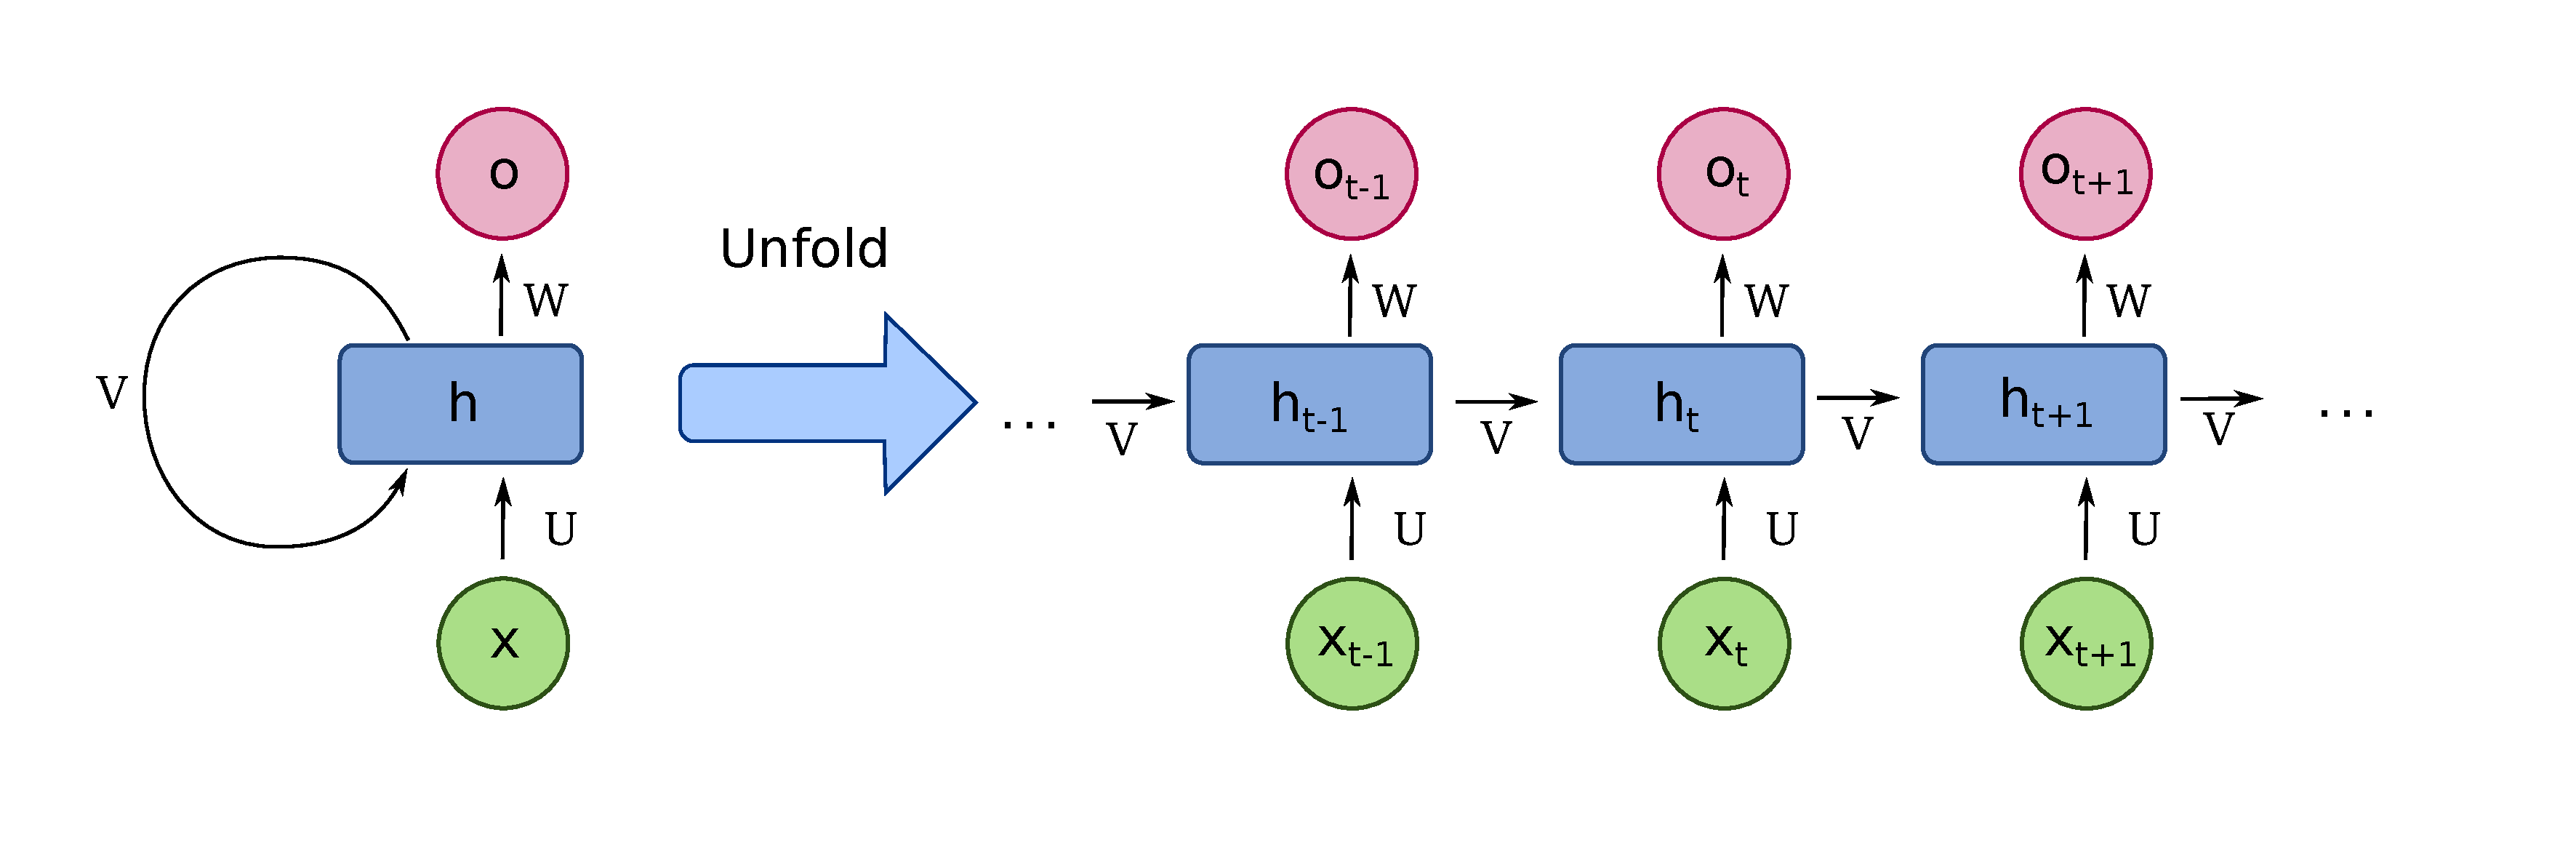
\includegraphics[width = 0.9\textwidth]{Imagenes/Vectorial/RNN_cell.pdf}
	\caption{Estructura de una neurona de una RNN}%https://en.wikipedia.org/wiki/Recurrent_neural_network
	\label{fig:RNN}
\end{figure}

Este tipo de redes se encarga de procesar la información de forma secuencial, es decir, la información pasa capa por capa en el mismo orden en que fue recibida, como se puede apreciar en la Figura \ref{fig:RNN}\footnote{Tomada de \url{https://en.wikipedia.org/wiki/Recurrent_neural_network}}. En las capas ocultas las neuronas se nutren de la información que le llega por la entrada, así como la información que había recibido previamente, consiguiendo así una cierta memoria, que utiliza, junto a la información de entrada, para predecir los resultados. 

Este tipo de redes tienen ciertos problemas, entre los que destaca el \textit{Vanishing/Exploding Gradients Problem}, identificado por \cite{hochreiter1991untersuchungen}.  Este problema dificulta el proceso de entrenamiento de las Redes Neuronales Recurrentes, haciendo que la red llegue a un estado de subajuste o que directamente no sea capaz de generalizar la información. El problema surge al acumular el resultado de los inputs previos, escalado con el peso correspondiente a la neurona, haciendo que en los casos en que el peso es menor que uno, la aportación de los estados previos resulte insignificante para los actuales y posteriores. Un problema análogo ocurre con los pesos mayores que uno.

Posteriormente surgen nuevos trabajos con el propósito de solucionar estos problemas. Entre estos tenemos como ejemplo el Long short-term Memory (LSTM)

\subsubsection{LSTM}

Este modelo (Long Short-term Memory) propuesto en \cite{hochreiter1997long}, es una evolución de las Redes Neuronales Recurrentes mencionadas anteriormente, que pretende solucionar el \textit{Vanishing/Exploding Gradient Problem}.

La solución que proponen tiene una mayor capacidad de recordar datos antiguos y se basa en ir decidiendo qué información olvidar a la vez que se considera al mismo tiempo el cúmulo de aprendizaje a corto y largo plazo.

\begin{figure}[h]
	\centering
	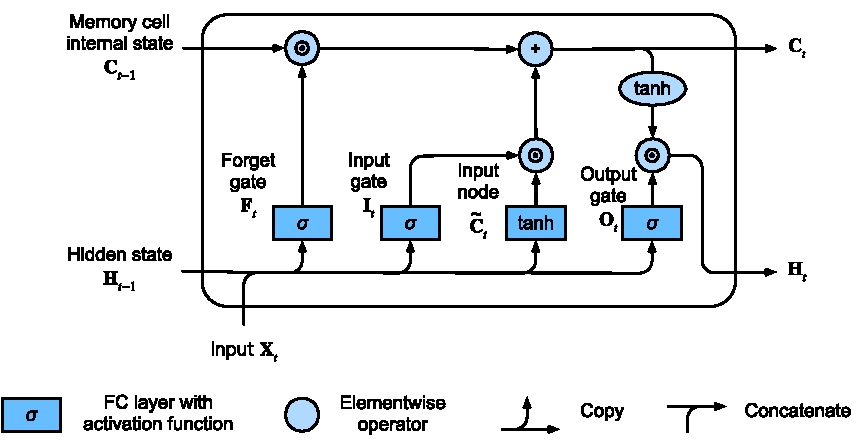
\includegraphics[width = 0.9\textwidth]{Imagenes/Vectorial/LSTM.pdf}
	\caption{Estructura de una celda LSTM}%Fuente: https://d2l.ai/chapter_recurrent-modern/lstm.html
	\label{fig:LSTM}
\end{figure}

Las Celdas de esta arquitectura están conformadas por cuatro tipos de puerta. Tenemos una ilustración en la Figura \ref{fig:LSTM}\footnote{Tomada de \url{https://d2l.ai/chapter_recurrent-modern/lstm.html}}
\begin{itemize}
	\item\textbf{Forget Gate} Se encarga de reajustar la información proveniente de estados antiguos en base al input recibido para decidir cuanta de esta seguirá teniendo en cuenta.
	\item\textbf{Cell state} Es el componente encargado de transportar la información a lo largo del tiempo.
	\item\textbf{Input Gate} Se encarga de decidir en qué medida influirá el input actual a los posteriores estados del sistema (memoria a largo plazo)
	\item\textbf{Output gate} Consigue el resultado final en base a la nueva memoria a largo plazo reajustada en combinación con el input y la memoria a corto plazo. Este resultado será la nueva memoria a corto plazo.
\end{itemize}

\subsubsection{Seq2Seq}

Fue propuesto en \cite{sutskever2014sequence}, con el propósito de resolver las dificultades que los modelos estadísticos presentaban a la hora de enfrentarse con la tarea de la traducción, concretamente la traducción de una secuencia de entrada a una secuencia de salida (Sequence 2 Sequence). Para lograr este propósito hacía uso del modelo presentado anteriormente, LSTM, junto a la arquitectura Encoder-Decoder. 

Este modelo se volvió relevante gracias a su mayor rendimiento, en comparación a los modelos estadísticos precedentes, en la tarea de la traducción de idiomas. Una de las razones por las que muestra un mayor desempeño, es que toma en consideración toda la secuencia de entrada para dar cualquier tipo de output. De esta forma es capaz de dar respuestas más coherentes con todo el contexto de la entrada.

\begin{figure}[h]
	\centering
	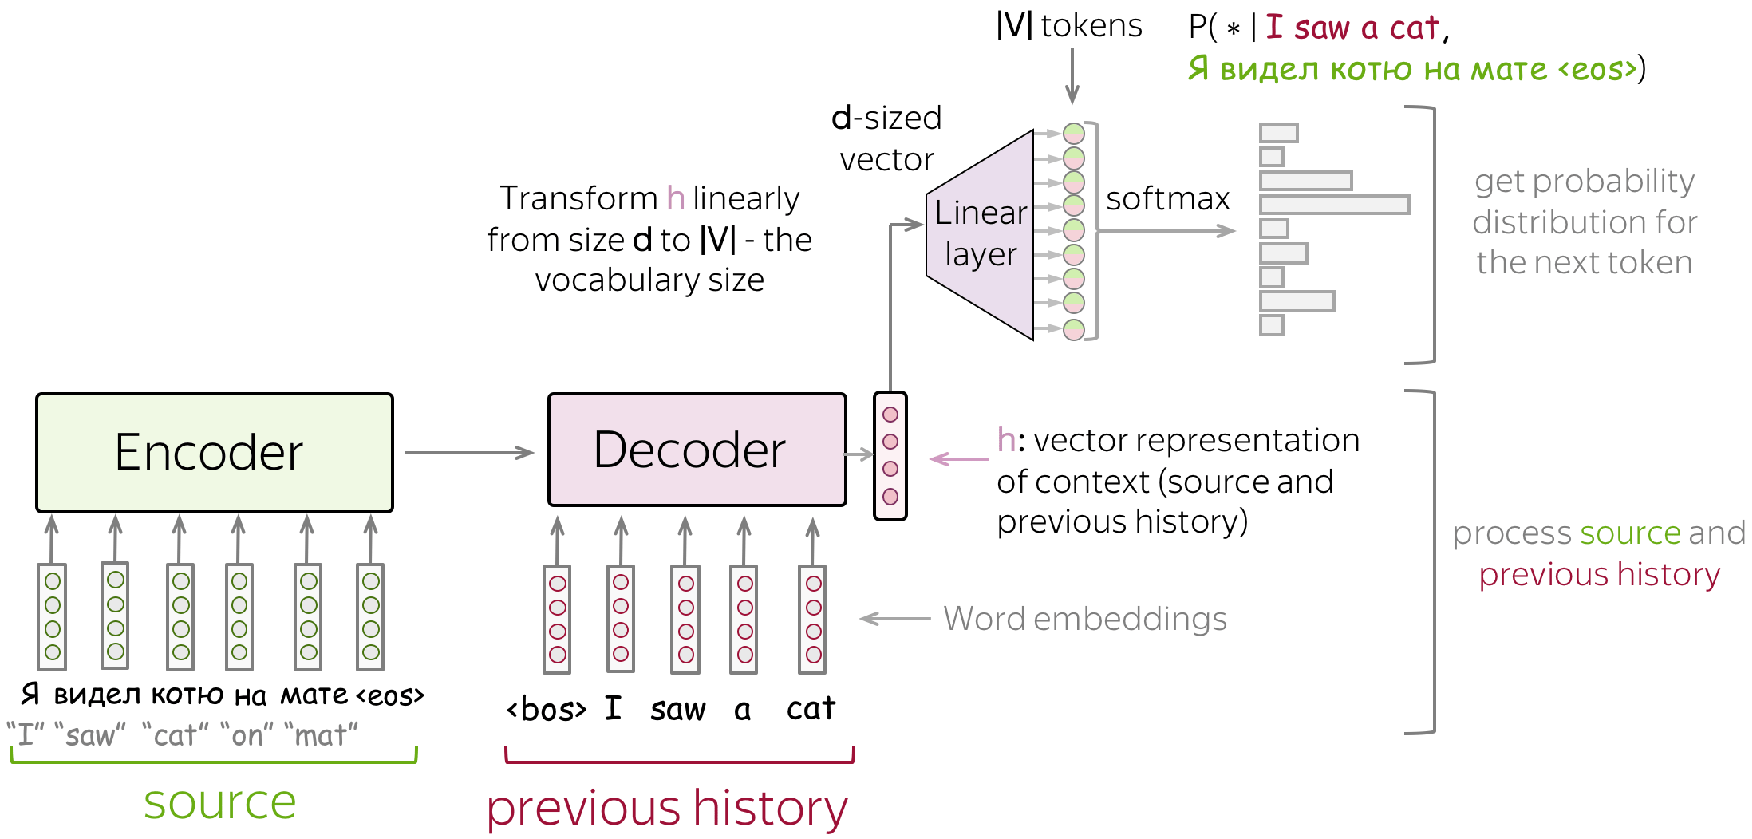
\includegraphics[width = 0.9\textwidth]{Imagenes/Vectorial/seq2seq.pdf}
	\caption{Estructura de una arquitectura seq2seq}%Fuente: https://lena-voita.github.io/nlp_course/seq2seq_and_attention.html
	\label{fig:seq2seq}
\end{figure}

La mayor novedad en este modelo es el uso de la arquitectura Encoder-Decoder. Continuamos con una breve explicación de los componentes principales de esta arquitectura, acompañados de una ilustración en la Figura \ref{fig:seq2seq}\footnote{Imáagen tomada de \url{https://lena-voita.github.io/nlp_course/seq2seq_and_attention.html}}:

\begin{itemize}
	\item \textbf{Encoder} Se encarga de tomar una secuencia de entrada y la transforma en una representación oculta de alta dimensión (\textit{Word Embeddings}), mediante el uso de una \textit{Embedding layer}, con esta representación se trata de capturar el contenido semántico de la oración recibida. A menudo los LSTMs son empleados como Encoders debido a su gran rendimiento al momento de manejar secuencias de datos largas y su capacidad de retentiva a lo largo del tiempo. En el estudio original \citep{sutskever2014sequence} en que se propuso el modelo seq2seq vemos que emplean 4 capas de 1000 celdas LSTMs cada una. Dejando en cada celda su propio conjunto independiente de pesos y sesgos. Y usando cada capa el Output de la capa anterior como Input.

Todo esto con el objetivo de producir el llamado \textit{Vector de Contexto}, que se usará como inicialización de memorias de corto y largo plazo para las capas de salida del decoder.

	\item \textbf{Decoder} Este se encarga de utilizar el \textit{Vector de Contexto} como memoria inicial tanto en el largo como corto plazo de sus capas de celdas LSTMs (en el paper \cite{sutskever2014sequence} emplean una red de LSTMs similar a la del decoder).

Para interpretar la información de salida de la última capa de celdas LSTMs, el Decoder utiliza un \textit{Word Embedding} correspondiente al \textit{lenguaje} de salida. Este obtiene su valor a partir de encadenar a la salida de la última capa LSTM una \textit{Fully Connected Layer} seguida de una función \textit{SoftMax} que se encargará de darnos finalmente el Output.

\end{itemize}

Este modelo soluciona varios de los problemas que surgían en modelos anteriores en el campo de la traducción, sin embargo se encuentra con sus propias limitaciones. Entre estas, la más importante, es el problema del \textit{Cuello de botella} que se ocasiona al tener que codificar todo el Input a través del Encoder para así obtener el \textit{Vector de Contexto} con el que inicializamos al Decoder. Otro de los problemas con los que se encuentra este modelo es el limitado contexto al que puede atender en la secuencia de entrada, esto se debe al hecho de que toda la secuencia de entrada se ha de representar mediante el \textit{Vector de Contexto}, llegando a perder mucha información en el caso de secuencias de entrada largas debido al tamaño fijo del \textit{Vector de Contexto}.

Poco después surge el trabajo \cite{bahdanau2014neural} que se centra en introducir los Mecanismos de atención, aliviando el problema de la limitiación en el tamaño de la secuencia de entrada.

Este mecanísmo consigue una mejor selección de la información tenida en cuenta por el \textit{Decoder} a la hora de decodificar la información del \textit{Encoder}. Esto lo hace a través de añadir, al \textit{Decoder}, mecanismos capaces de deducir la similitud entre las repsuestas ofrecidas por el \textit{Encoder} y el \textit{Decoder}.
\newpage
\subsubsection{Transformers}

Uno de los puntos de inflexión llega con el trabajo \cite{vaswani2017attention} presentado por investigadores de Google, que introduce multitud de conceptos, que, en conjunto, son capaces de ofrecer un modelo superior en rendimiento y desempeño a los anteriores. Una característica principal es el nuevo enfoque que dá, dejando de ser un nuevo paso en el camino trazado por los modelos explicados anteriormente, y proponiendo un modelo que pone la tilde en el mecanismo de atención y construyendo, a partir de este, un sistema capaz, de forma intrínseca, de atender a las relaciones semánticas entre los componentes de las secuencias tratadas (e.g. las palabras de un texto), además de ofrecer la posibilidad de realizar todas las tareas de entrenamiento e inferencia de una forma paralela, abriendo así la posiblidad a un aumento en la escala de este tipo de modelos como no se había visto y en el que aún no terminamos de ver el progreso. Ilustración en la Figura \ref{fig:Transformer Architecture}

\begin{figure} [hb]
	\centering
	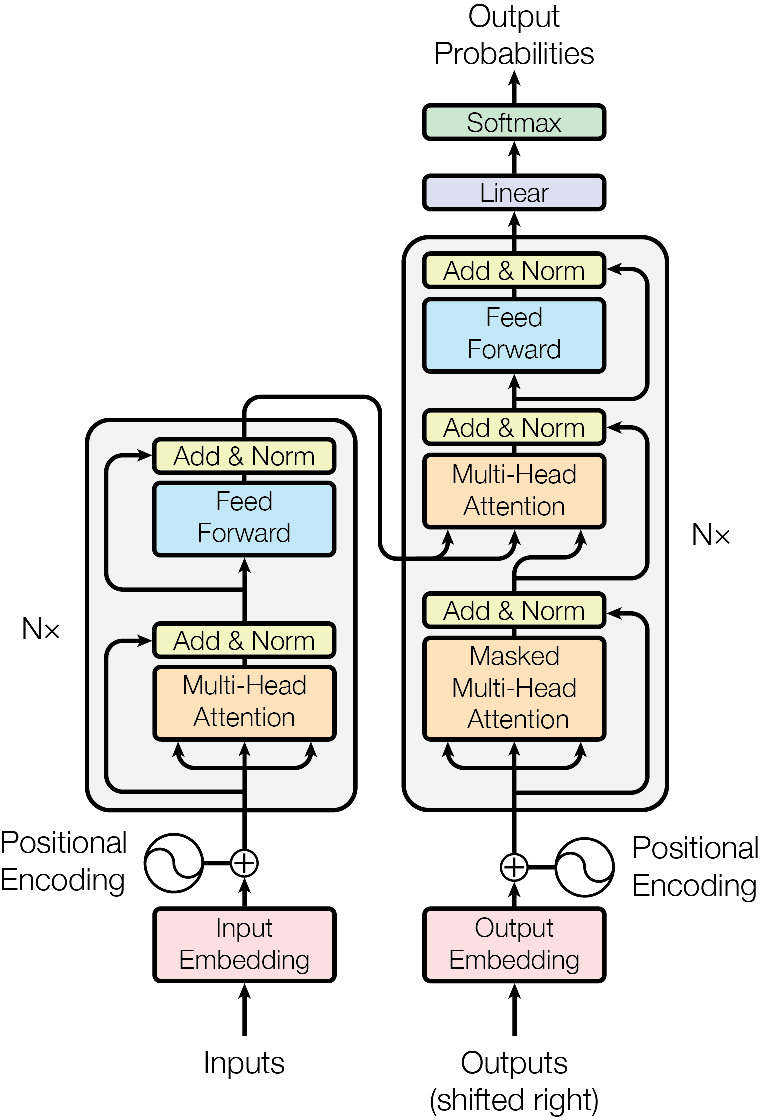
\includegraphics[width = 0.6\textwidth]{Imagenes/Vectorial/Transformer.pdf}
	\caption{Arquitectura Transformer (Imagen tomada de \cite{vaswani2017attention})}%Fuente: vaswani2017attention
	\label{fig:Transformer Architecture}	
\end{figure}

Entre los principales componentes con los que cuenta el modelo propuesto tenemos:\newpage
\begin{itemize}

\begin{figure} [hb]
	\centering
	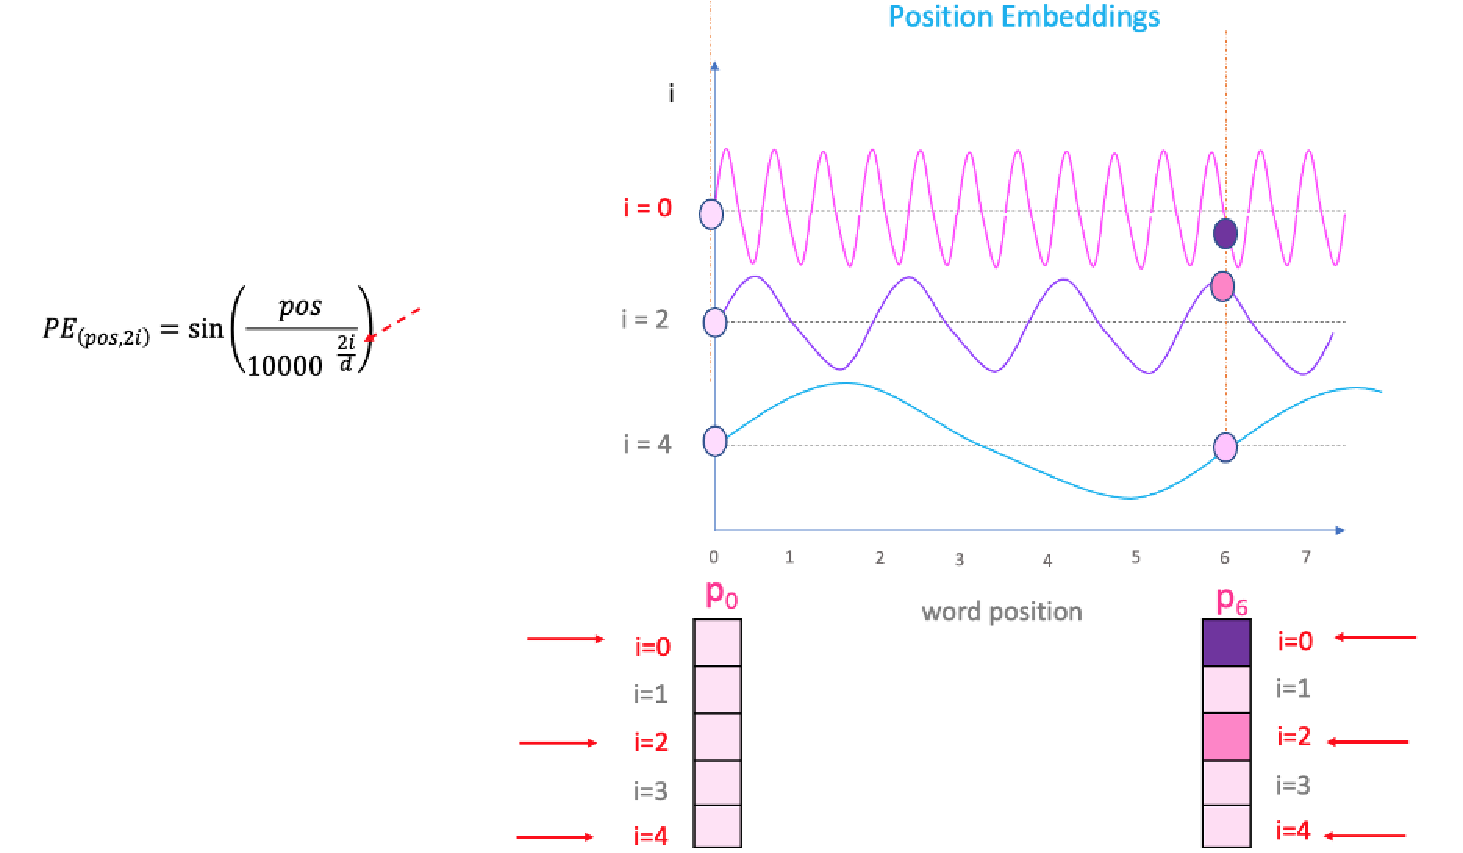
\includegraphics[width = 0.9\textwidth]{Imagenes/Vectorial/PositionalEncoding.pdf}
	\caption{Visualización del mecanismo \textit{Positional Encoding}}%Fuente: https://datascience.stackexchange.com/questions/51065/what-is-the-positional-encoding-in-the-transformer-model
	\label{fig:Positional Encoding}
\end{figure}

	\item\textbf{Positional Encoding} Como ya habíamos visto en varios modelos anteriores, a la hora de tratar las secuencias de entrada estas eran convertidas en Tokens correspondientes a un \textit{Word Embedding} con la intención de atrapar el significado semántico.

En este trabajo se añaden mecanismos para atrapar, a la vez que el significado semántico, la relación de orden de aparición entre los Tokens de la secuencia de entrada. Esto lo consiguen mediante la adición de los valores de funciones seno y coseno de frecuencias variando en función de la posición del Token y del tamaño del \textit{Word Embedding} permitiendo, además, atrapar esta relación de posición para cualquier longitud de cadena de entrada.

\[PE_{pos,2i} = \sin(pos/10000^{2i/d_{model}})\]
\[PE_{pos,2i+1} = \cos(pos/10000^{2i/d_{model}})\]

Podemos ver cómo actúa el mecanismo mediante la Figura \ref{fig:Positional Encoding}\footnote{\url{https://datascience.stackexchange.com/questions/51065/what-is-the-positional-encoding-in-the-transformer-model
}}. Donde se ilustra en qué forma varía la codificación en relación a la posición del Token.

	\item\textbf{Self Attention} Busca la similaridad entre una palabra con todas las demás, y con ella misma. Actúa sobre la secuencia de entrada para asignar la importancia que cada una de estas tiene en la palabra en la que nos habíamos enfocado inicialmente (producto escalar). Para lograr esto introduce con cada palabra tres nuevos valores \textit{Query}, \textit{Key} y \textit{Value}, con el objetivo de lograr una codificación para cada palabra resultado de su relación con las demás, que es el que usará como valor representativo del Token (ver figura \ref{fig:Scaled Dot-Product Attention}).

El uso que se le da al valor \textit{Query} es obtener a través de este y todos los demás valores \textit{Key} una serie de valores con la que, al pasar por una función \textit{Softmax}, obtenemos el peso que damos a cada uno de los valores \textit{Value} de los otros Token, consiguiendo con la suma de todo esto el valor que esperábamos para la palabra de la que empleábamos el \textit{Query}.

Una gran ventaja de este mecanismo es la paralelización que ofrece en la fase de codificación, ya que para el cálculo del valor de codificación no necesitas ningún resultado dependiente de las palabras anteriores. Eliminando el problema que tenían modelos anteriores en la obtención del \textit{Vector de Contexto}.

La arquitectura puede tener multiples capas de atención. Capturando cada una de ellas distintas relaciones entre las palabras y de forma completamente independiente y paralelizable (ver Figura \ref{fig:Multi-Head Attention}).

\begin{figure}
	\begin{minipage}[b]{0.5\linewidth}
		\centering
		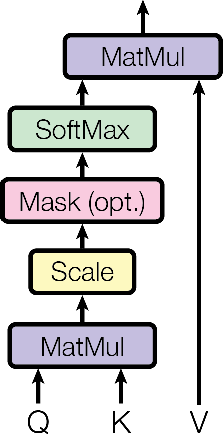
\includegraphics[width=0.5\linewidth]{Imagenes/Vectorial/ScaledDotProduct.pdf}
		\caption{Ilustración del mecanismo de \textit{Self-Attention}. Tomada de \cite{vaswani2017attention}}%Fuente: vaswani2017attention
		\label{fig:Scaled Dot-Product Attention}
	\end{minipage}
	\begin{minipage}[b]{0.5\linewidth}
		\centering
		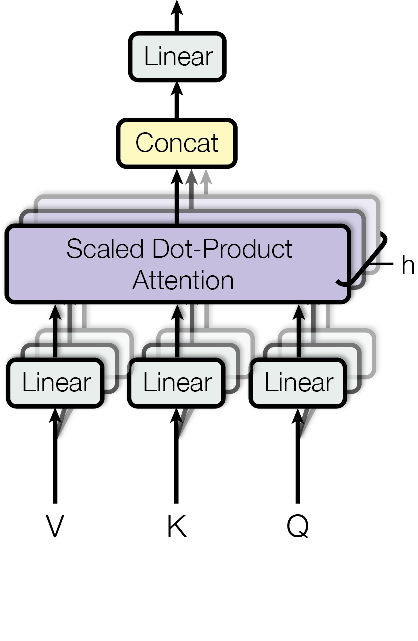
\includegraphics[width=0.5\linewidth]{Imagenes/Vectorial/MultiHeadAttention.pdf}
		\caption{Ilustración de múltiples capas en la fase de atención. Tomada de \cite{vaswani2017attention}}%Fuente: vaswani2017attention
		\label{fig:Multi-Head Attention}
	\end{minipage}
\end{figure}

Además permite añadir múltiples capas con pesos y desvios distintos, de forma que la arquitectura sea capaz de enfocarse en varios tipos de relaciones entre las palabras. En el trabajo presentado por Google propusieron un modelo con 8 capas.

\end{itemize}

Con este último modelo hemos hecho un repaso de la evolución que este campo ha sufrido. Partiendo de modelos formalizados hace más de 4 décadas hasta modelos propuestos hace menos de 5 años y que actualmente nutren las arquitecturas propuestas para llevar a cabo la construcción de sistemas tan presentes y capaces en nuestro día a día. Tenemos ejemplos claros en productos como ChatGPT o la competición que se está viendo en el campo de los LLM involucrando a empresas de primer calibre como Microsoft, Meta, Google u OpenAI, ofreciendonos tanto modelos como asistentes de chat nuevos y más potentes cada pocos meses. Este tipo de modelos es el que más desarrollos ha sufrido y todos ellos se basan en la arquitectura que acabamos de presentar.

\subsection{Grandes Modelos de Lenguaje}

Como hemos visto en la sección anterior, una de las grandes ventajas de los Transformers fué la paralelización, abriendo el paso al desarrollo de modelos cada vez más grandes y versátiles. Esta versatilidad ha hecho buscar en este tipo de modelos infinidad de aplicaciones. Sin embargo, esta capacidad viene acompañada de una alta necesidad de cómputo para llevar a cabo un entrenamiento, haciendo muy restrictivo el acceso a dichos modelos. Es por ello que este tipo de tecnologías han sido abordadas por entidades con una gran cantidad de recursos computacionales, como ejemplo Google que introdujo la arquitectura BERT o GPT introducida por OpenAI. Aunque  en ocasiones estos avances se compartían de forma abierta (\cite{touvron2023llama}) y hay multitud de iniciativas que abogan por el desarrollo libre, 

\subsection{Generativos}

\section{Procesamiento del lenguaje natural}

El procesamiento del lenguaje natural (PLN) es una rama de la inteligencia artificial que se enfoca en la interacción entre las computadoras y el lenguaje humano. El objetivo del PLN es permitir que las máquinas comprendan y procesen el lenguaje humano de la misma manera que lo hacemos los seres humanos. Esto lo consiguen combinando la lingüística computacional con modelos estadísticos de machine learning y deep learning, pudiendo así interpretar tanto datos de texto como de voz, e incluso imágenes u otros tipos.

\subsection{Historia del PLN}

Se podría considerar el 1950 como el año de surgimiento del PLN, con la publicación de \cite{10.1093/mind/LIX.236.433}, donde se proponía el conocido \textit{Test de Turing}, una herramienta que evalúa la capacidad de una máquina para exhibir un comportamiento inteligente similar o indistinguible al de un ser humano, teniendo a una persona como evaluadora del comportamiento y comparando las respuestas con las de un humano real. Esto abrió el debate sobre si las máquinas eran o no capaces de ''pensar'' y sobre cómo pueden interpretar el texto que reciben y devolver una salida que cobre sentido.

Entre finales de los años 70 y el año 1985, surgieron modelos que se basaban en reglas para realizar traducciones automáticas, ya que en la época, era el principal objetivo del PLN, como Syntra \citep{Toma1970SYSTRANMT}. A principios del siglo XXI se vio que estos sistemas no eran los más eficientes y, a partir de los años 2010, se empezó a emplear el método de la inteligencia artificial para el procesamiento del lenguaje natural.

En la actualidad, las investigaciones en PLN se centran en mejorar la capacidad de las máquinas para comprender el contexto y la intención detrás del lenguaje humano. Avances notables incluyen el desarrollo de modelos de lenguaje preentrenados, como BERT (Bidirectional Encoder Representations from Transformers) y GPT (Generative Pre-trained Transformer), que han demostrado una capacidad excepcional para captar la complejidad del lenguaje natural \citep{devlin2019bert}.

A día de hoy, estos sistemas han sido perfeccionados y se utilizan de manera habitual en varios ámbitos como pueden ser la recuperación y extracción de información, la minería de datos, la traducción automática, el análisis de sentimientos o la generación de resúmenes automáticos \citep{hernandez2013aplicaciones}. En el caso de este estudio, es especialmente interesante la generación de resúmenes automáticos, ya que es una de las extensiones propuestas en los objetivos de realización del trabajo.

\subsection{PLN para resúmenes de textos}

En los últimos años, se han propuesto diversos generadores de secuencias. En particular, los que más éxito han tenido son los basados en arquitecturas de aprendizaje profundo (deep learning) \citep{mishra2020deep}. Las definiciones de la figura \ref{fig:resumenTextos} se refieren a los distintos tipos de resúmenes de textos que pueden existir, según \cite{adhikari2020nlp}. 

\begin{figure}[h]
	\centering
	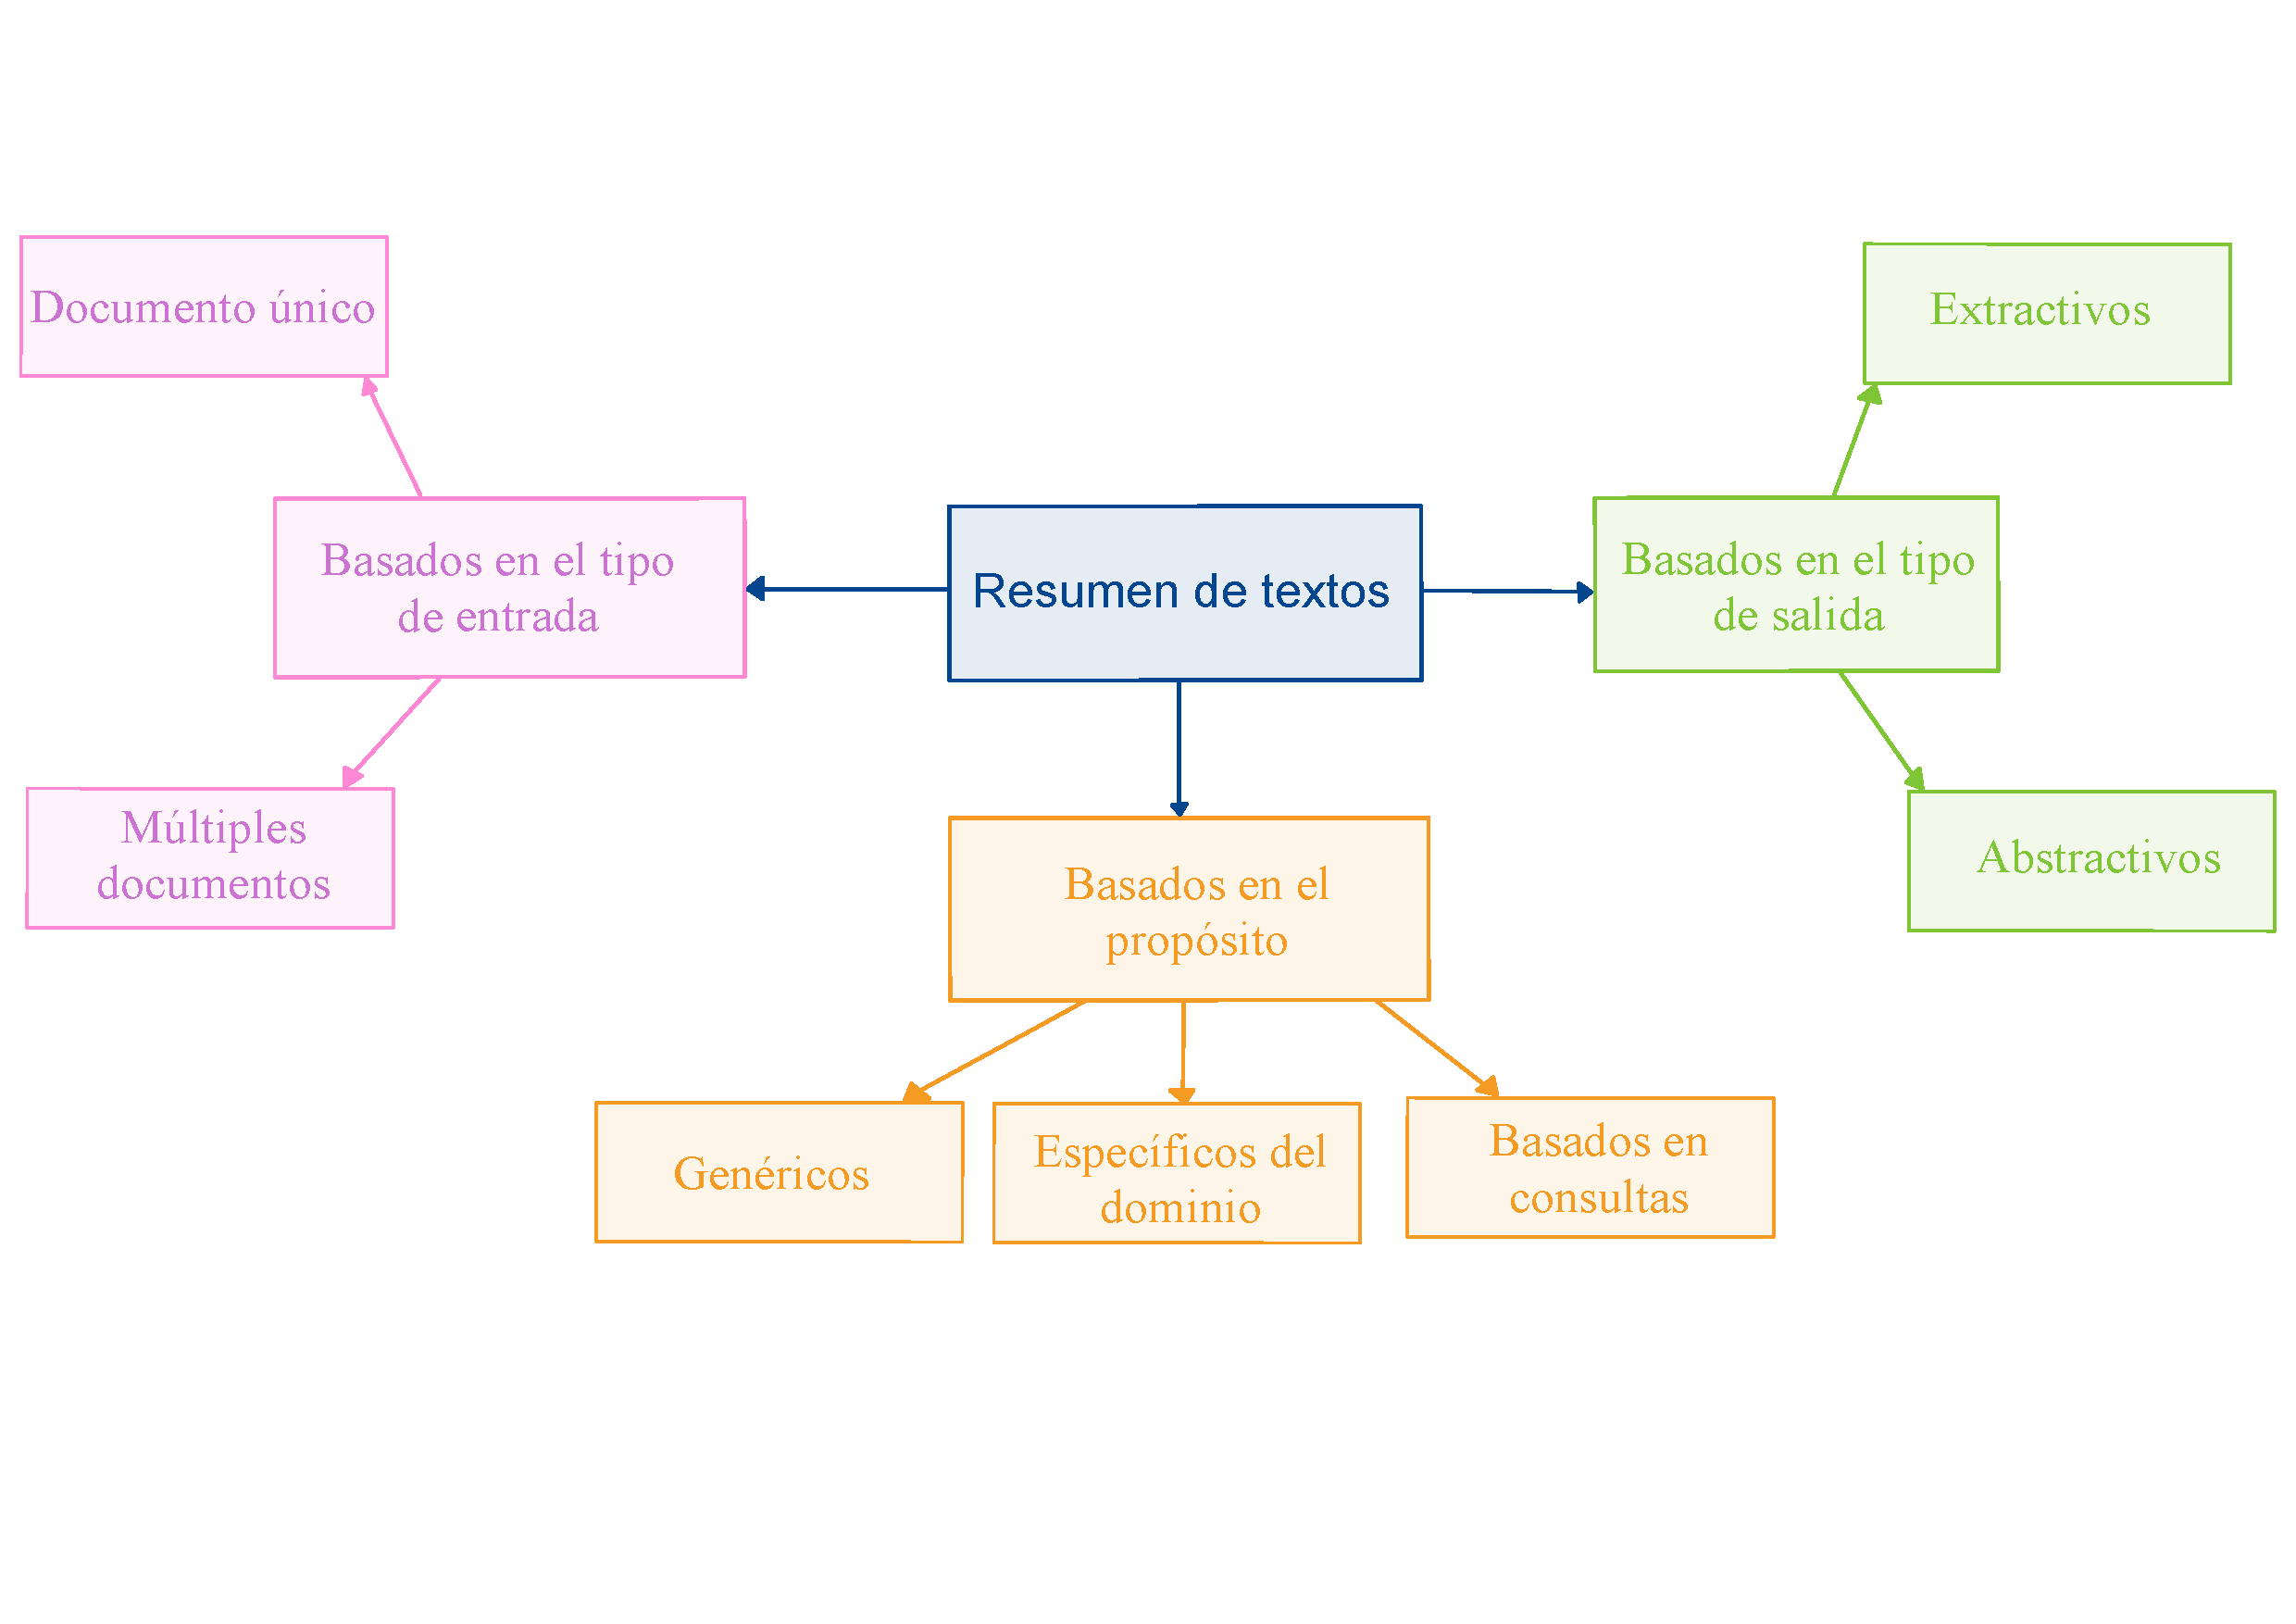
\includegraphics[width = 0.7\textwidth]{Imagenes/Vectorial/resumenTextos.pdf}
	\caption{Resumen de textos (adaptada de \cite{adhikari2020nlp})}
	\label{fig:resumenTextos}
\end{figure}

Los resúmenes extractivos son los que reutilizan las mismas frases existentes en el documento original, los abstractivos son más generales y se centran en los aspectos clave. De manera similar, las técnicas de resumen de un solo documento proporcionan resúmenes del texto de un solo documento, y las de múltiples documentos, generan resúmenes de varios documentos. Además, en la actualidad, hay una necesidad de resumir texto basándose en consultas. Los modelos de resumen basados en consultas proporcionan resúmenes del texto según un área específica descrita por la consulta proporcionada por el usuario, mientras que los resúmenes genéricos son en su mayoría resúmenes abstractos que se centran en el área general del texto de entrada.

\subsection{Impacto del desarrollo del PLN en la sociedad actual}

Como se ha visto, el procesamiento del lenguaje natural se ha desarrollado enormemente desde su concepción, especialmente en los últimos años. Con el uso de las tecnologías más modernas, se ha conseguido que el PLN sea parte del día a día de una persona común, lo cual ha traido múltiples beneficios a la sociedad, como pueden ser los siguientes:

\begin{itemize}
	\item \textbf{Mejora en la comunicación}: Facilitando la interacción con dispositivos electrónicos, como pueden ser los asistentes virtuales conocidos como Siri (de Apple) o Alexa (de Amazon). Además, al interpretar el lenguaje natural, se han creado diferentes dispositivos que permiten a personas con discapacidades, comunicarse con otra gente.
	
	\item \textbf{Progreso de la traducción automática}: Como se ha visto, la traducción automática tanto de discursos como de textos ha sido uno de los puntos de estudio principales relacionados con el PLN. A día de hoy, este ámbito está bastante desarrollado y permite unir personas de diferentes culturas y países.
	
	\item \textbf{Ayudas de soporte para negocios}: Con la proliferación de los conocidos 'chatbots', muchos negocios de todos los tamaños se han visto beneficiados, pudiendo incorporarlos como una medida de soporte para los clientes.
	
	\item \textbf{Análisis avanzado de datos}: El PLN permite utilizar enormes cantidades de texto y aportar estadísticas importantes a partir de él, lo cual sería muy difícil para os humanos debido a las grandes cantidades de información. Además, estos análisis a gran escala pueden servir para analizar los sentimientos de los mensajes publicados en redes sociales, por ejemplo.
\end{itemize}

A pesar de todas estas ventajas que el procesamiento del lenguaje natural ha aportado a la sociedad, existen varios desafíos para que esta tecnología sea capaz de funcionar. Las máquinas requieren una comunicación precisa y exacta, y los humanos hablamos con ambigüedades y de forma poco precisa en el día a día. Además, para poder transcribir a texto las palabras de una persona, es necesario un uso claro y comprensible del lenguaje. Estas solo son algunas de las barreras en las que se está trabajando para poder hacer esta tecnología accesible a todo el mundo.


\section{Computación centrada en el humano}

La computación centrada en el humano (CCH) es una disciplina que se dedica a  centrar todo el desarrollo de un sistema informátivo en los seres humanos que la usarán, así como estudiar los fenómenos relacionados más significativos. Para esto, la CCH incorpora en sus estudios varios factores humanos en el diseño y prácticas de la informática, como pueden ser circunstancias sociales o culturales, empleando para ello equipos multidisciplinares para resolver los desafíos, más que equipos puramente tecnológicos.

Este tema es abordado desde hace muchos años, analizando el artículo de \cite{Card1983ThePO}, vemos que estos abogan por una perspectiva que no solo se centre en la eficiencia técnica del sistema, argumentando que ''un buen diseño de sistema se debe evaluar en términos de la eficacia con la cual el sistema ayuda a los usuarios a alcanzar sus metas''. Lo cual subraya la importancia de no solo medir el éxito de un programa informático en términos de rendimiento, sino también en la capacidad del sistema para ser comprensible, usable y facilite las tareas del humano que lo usa.

Además, otro de los objetivos de la computación centrada en el humapno es crear sistemas que sean adaptables a los requerimientos cambiantes del usuario. No es solamente hacer un sistema optimizado y usable por los humanos, sino que también se pueda amoldar a las necesidades cambiantes de los futuros usuarios.

\subsection{Interacción Persona-Ordenador }

La Interacción Persona-Ordenador (IPO) es un área más específica que la computación centrada en el humano, ya que esta se focaliza especialmente en la relación entre el sistema y el humano, y no se centra tanto en factores externos más globales.

Los ordenadores llegaron a nuestras vidas en la década de 1940, y la ciencia de la interacción entre las personas y ordenadores llegó en la década de 1980. Entonces, ¿entre 1940 y 1980 no había interacción entre personas y ordenadores? No exactamente. En aquellas épocas, los ordenadores no estaban tan masificadamente disponibles como lo están a día de hoy, por lo que solo un selecto grupo de personas podían ''comunicarse'' con ellos. Estas personas eran perfiles técnicos como ingenieros y científicos, por ello la interacción era muy compleja y un amplio conocimiento técnico era necesario. \citep{mackenzie2012human}.

A partir de la década de 1980, con la llegada de los ordenadores a la vida cotidiana de las personas, se comenzó a investigar acerca de cómo facilitar la accesibilidad a todos los públicos para interactuar con las máquinas.  La investigación en el campo de la IPO ha abordado una amplia gama de aspectos, desde la usabilidad y la experiencia del usuario hasta la accesibilidad y la adaptabilidad de los sistemas informáticos.

La usabilidad, en particular, ha sido un tema central en la IPO. Este concepto se refiere a la facilidad con la que los usuarios pueden aprender a utilizar un sistema, realizar tareas y recordar cómo usarlo en el futuro. Uno de los estudios más importantes en este campo es el de Jakob Nielsen \cite{nielsen1994usability}, en el que identifica los principios como la visibilidad del estado del sistema o la correspondencia entre el sistema y el mundo real como elementos clave para mejorar la usabilidad de los sistemas informáticos.

Además de la usabilidad, la experiencia de usuario (UX por sus siglas en inglés) también ha sido un área de interés en este ámbito. La UX se refiere a las percepciones y respuestas de una persona que resultan del uso o de un producto, sistema o servicio. En resumen, el estudio de las vivencias de los usuarios con el programa informático. Don Norman, en su libro \cite{norman2013design}, introdujo el concepto de ''diseño centrado en el usuario'', donde enfatizó la importancia de diseñar productos que se alineen con la forma en que las personas piensan.

\subsection{Proceso de diseño centrado en el humano}

El diseño centrado en el humano es un enfoque de desarrollo de productos (en nuestro caso, de software) que pone al usuario en el centro del proceso de diseño. Reconoce la importancia de comprender las necesidades, capacidades y preferencias de los usuarios finales.

El proceso de diseño centrado en el humano generalmente sigue una serie de etapas iterativas que incluyen investigación, diseño, prototipado, evaluación y refinamiento.

La investigación de usuarios es una etapa fundamental. Esta etapa implica la recopilación y análisis de información sobre los usuarios finales, incluyendo sus características demográficas, necesidades, comportamientos y preferencias.

Basándose en los hallazgos de la investigación de usuarios, los diseñadores pasan a la etapa de diseño conceptual, donde generan ideas y conceptos de diseño que abordan las necesidades y metas identificadas de los usuarios. En esta etapa se suelen crear prototipos de baja fidelidad, como bocetos y maquetas, para explorar ideas de manera rápida y económica.

Los siguientes pasos son los de prototipado y evaluación, donde se crean prototipos de alta fidelidad que simulan la funcionalidad y la apariencia del producto final. Estos prototipos se someten a pruebas de usabilidad y evaluaciones de usuario para identificar problemas y áreas de mejora.

Finalmente, basándose en los resultados de la evaluación, los diseñadores refinan y mejoran el diseño del producto, iterando en el proceso según sea necesario. Este enfoque iterativo permite a los diseñadores incorporar el feedback de los usuarios y abordar los problemas de diseño de manera proactiva, creando productos que se alinean mejor con las necesidades y expectativas de los usuarios finales.

\subsection{Computación afectiva}

La computación afectiva es el estudio y desarrollo de sistemas y dispositivos que reconocen, interpretan, procesan y simulan el afecto humano. Está muy relacionada con la computación centrada en los humanos, ya que hace especial hincapié en las emociones de los humanos al desarrollar sistemas informáticos. Esta rama de la computación se corresponde a un campo interdisciplinar que abarca tanto las ciencias de computación, psicología y ciencias cognitivas. Esta ciencia comenzó a ser analizada a partir del artículo científico publicado de \cite{picard1995computer}, en el cual se estudiaban maneras de aplicar la subjetividad humana a los computadores.

Dos de las áreas de la computación afectiva son la detección y reconocimiento de información emocional y la emoción en las máquinas. La primera área comienza con sensores que capturan datos sobre el estado físico o comportamiento de la persona, sin interpretar los datos de entrada. Estos sensores son análogos a las técnicas que utilizan los humanos para detectar las emociones en otras personas (expresiones faciales, posturas, temperatura corporal, etc.). En cuanto al área de la emoción en las máquinas, se estudia la capacidad que tienen estos computadores de convencer y simular emociones humanas. En el libro de \cite{minsky2007emotion} se propone que las emociones "no con específicamente tan diferentes de otros procesos a los que consideramos 'pensamiento'", por lo que podría ser que estas lleguen a simular sentimientos mediante un proceso de lógica.

\subsection{Ejemplos reales de CCH }

El campo de la computación, existen varios temas del mundo real a los que se puede aplicar, algunos ejemplos de esto son los siguientes:

\begin{itemize}
	\item \textbf{Solución de problemas en entornos distribuidos}: Abarcando sistemas de información basados en Internet, redes de información basadas en sensores o dispositivos de información móviles y vestibles (relojes inteligentes, por ejemplo). Todos estos sistemas han de ser diseñados considerando al humano como centro del estudio.
	
	\item \textbf{Sistemas multi-agente} que controlan y coordinan acciones para resolver problemas complejos, como es el caso en el que nos basamos para el presente trabajo, extendiendo y adaptando el sistema multi-agente desarrollado en es estudio de \cite{park2023generative}.
	
	\item \textbf{Definición de estructuras semánticas} para que la información multimedia dé soporte a entradaas y salidas de múltiples modalidades. Como se ha visto en el apartado anterior de PLN, este campo es muy importante para la democratización a todos los públicos y que se está promoviendo en los avances actuales de la tecnología.
	
\end{itemize}

Además, existen casos de proyectos reales en los que se está aplicando la CHH, uno de ellos es la División de Ciencias Computacionales NASA/Ames, la cual está realizando una investigación como miembros del Proyecto Haughton-Mars para determinar, vía estudio de analogías, cómo de probable es que la vida humana sea fructífera en Marte. Uno de las investigaciones dentro de este proyecto es el desarrollo de robots que asistirán a los científicos, ayudándoles a tomar en consideración los factores humanos, de computación y del entorno para poder sobrevivir en Marte.

Otro de los ejemplos es el Centro de Computación Cognitiva Ubicua (CUbiC) de la Universidad Estatal de Arizona, el cual se basa en los principios de la CCH para desarrollar aplicaciones asistivas, rehabilitativas y de salud. Algunos ejemplos de estos desarrollos son los conocidos como 'Note-Taker', un dispositivo diseñado para ayudar a los estudiantescon poca visión a seguir las clases y tomar apuntes, o el 'VibroGlove', que reconoce las expresiones faciales mediante retroalimentación háptica para ayudar a personas con problemas visuales.

\section{Relaciones sociales}

El artículo de \cite{park2023generative} sobre el que se ha basado la realización de este trabajo de fin de grado, está muy enfocado en el estudio del comportamiento humano y las finalidades que podría tener el hecho de simular relaciones sociales entre agentes de inteligenicia artificial. Algunos de los casos de uso de este estudio podrían ser la incorporación a personajes no jugables en videojuegos o la simulación de entornos reales para ver cómo afectaría la introducción de cambios en el ambiente, tal y como se menciona en el artículo.

Sin embargo, las relaciones sociales son un tema importante en la psicología y se han estudiado desde diferentes perspectivas. En la informática, el estudio de las relaciones sociales se ha centrado en la creación de sistemas que permitan la interacción social en línea. Es por eso que se divide el estudio de las relaciones sociales en estos dos campos, abordando en cada uno el contexto, la historia e investigaciones anteriores relacionadas con las relaciones sociales desde dos ámbitos diferentes.

\subsection{Psicología}

Las relaciones sociales desempeñan un papel fundamental en la vida humana, impactando de manera significativa en el bienestar emocional y mental de las personas. El estudio de las interacciones sociales ha revelado una serie de beneficios intrínsecos que estas conexiones ofrecen a nivel psicológico y emocional.

A lo largo del tiempo ha habido estudios que muestran de manera consistente que los individuos con menor cantidad de relaciones sociales son mas propensos a fallecer en comparación con lo que tienen una vida social plena. Estos estudios han arrojado una mayor evidencia en países industrializados \citep{House1988}.

Una vez se conoció el claro vínculo entre las relaciones sociales y la salud de las personas, los científicos se centraron en explicar cómo ocurre esto. Generalmente, existen tres amplias maneras en las que las relaciones sociales influencian la salud: de comportamiento, psicosociales y fisiológicas \citep{doi:10.1177/0022146510383501}.

\begin{itemize}
	\item \textbf{Explicaciones de comportamiento}: 
	Los comportamientos relacionados con la salud abarcan una amplia gama de conductas personales que influyen en la salud, la morbilidad y la mortalidad. De hecho, los comportamientos relacionados con la salud explican aproximadamente el 40 por ciento de la mortalidad prematura, así como una morbilidad y discapacidad sustanciales en los Estados Unidos. \citep{activePolicyAttention}
	
	\item \textbf{Explicaciones psicosociales}: La investigación en diferentes disciplinas y poblaciones sugiere la posibilidad de que algunos mecanismos psicosociales influyan en como los lazos sociales promueven la salud. Diferentes estudios han observado solamente uno de estos mecanismos, pero debido a la complejidad de la interconexión de estos mecanismos, hace que no sea posible llegar a una conclusión certera a no ser que se estudien todos a la vez.
	
	\item \textbf{Explicaciones fisiológicas}: Profesionales de varios ámbitos del mundo de la salud han  contribuido al entendimiento de algunas acciones (consumo excesivo de comida, de alcohol, de tabaco...) para reducir el estrés. Además, estas acciones muchas veces están relacionadas con actividades sociales y, el hecho de relacionarse con gente que exceda el consumo de estas sustancias, puede afectar gravemente a la salud.
	
	
\end{itemize}

Se ha visto que las relaciones sociales pueden ser muy positivas para la salud; sin embargo, también se ha comprobado que las relaciones sociales de mala calidad, también pueden afectar de manera negativa en la salud de las personas. Un matrinonio con problemas de comunicación o de entendimiento se ha asociado con funciones del sistema inmune o endocrino afectadas \citep{doi:10.1177/0265407500171001}.

\subsection{Informática a lo largo del tiempo}

El estudio de las relaciones sociales en el ámbito de la informática ha abarcado una amplia gama de temas, desde la privacidad y la seguridad en línea hasta la influencia de las redes sociales en la política y la sociedad. Además, con la aparición de las inteligencias artificiales, últimamente también se ha investigado sobre el grado de independencia que puedan tener, o cómo de humanas se pueden sentir. También se especula por cómo de cerca está la humanidad de alcanzar a construir una inteligencia artificial general (AGI por sus siglas en inglés). Esta AGI tendría un razonamiento indistinguible del de un ser humano y una capacidad de cálculo de una máquina, por ello este tema del comportamiento humano es tan estudiado para el desarrollo de nuevas IAs.

Para el caso del presente trabajo, es especialmente interesante el análisis de comportamientos humanos en agentes de inteligencia artificial. Esto es un campo que se lleva considerando más de 20 años, con el estudio de \cite{CASTELFRANCHI1998157}. Ya en este estudio se trata de probar la emergencia de fenómenos sociales, así como la cooperación entre diferentes agentes (eso sí, con una tecnología muy inferior a la actual).

Años más tarde, se publica otro estudio con un propósito similar \citep{pan2007multi}. En este caso la intención era simular comportamientos humanos en la evacuación de emergencias. Esto revela un nuevo paradigma en el que se puede aplicar este tipo de estudio. Si se consiguen unos agentes independientes capaces de interrelacionarse entre sí, estos podrían adquirir ciertos roles y representar situaciones reales de cómo actuarían humanos con esas características en esas situaciones. En el caso de las evacuaciones de emergencia esto ayuda mucho ya que se podrían evitar catástrofes mayores.

En un estudio más reciente \citep{benvenuti2023artificial} se investiga sobre el modelado del comportamiento humano tras la irrupción de las inteligencias artificiales. Se explica que se necesita mayor investigación en esta área, prestando especial atención a la educación primaria. En el artículo se defiende que la educación debería pivotar y en lugar fomentar una cultura de sabiduría, se debería fomentar una cultura de la competencia. Esta es una de las maneras en las que las tecnologías informáticas modelan el comportamiento humano para adaptarse a las nuevas tecnologías.

Además de estos ejemplos en los que se estudian las relaciones sociales y comportamientos humanos relacionados con la inteligencia artificial, uno de los mayores avances de la humanidad en cuanto a la interconexión y fomento de las relaciones sociales a distancia fueron las redes sociales.

\subsubsection{Redes Sociales}

Las redes sociales se han convertido en una parte integral de la vida en línea. Estas permiten a los usuarios conectarse con amigos y familiares, compartir información y contenido, y participar en comunidades en línea. Esto favorece por tanto las relaciones sociales a distancia usando las tecnologías de la informática.

En 1997, Andrew Weinreich creó el sitio web 'SixDegrees.com', que se considera la primera red social de la historia, en la cual los usuarios podían configurar su página de perfil, crear listas de ocnexiones y enviar mensajes entre sus contactos.

\begin{figure}[h]
	\centering
	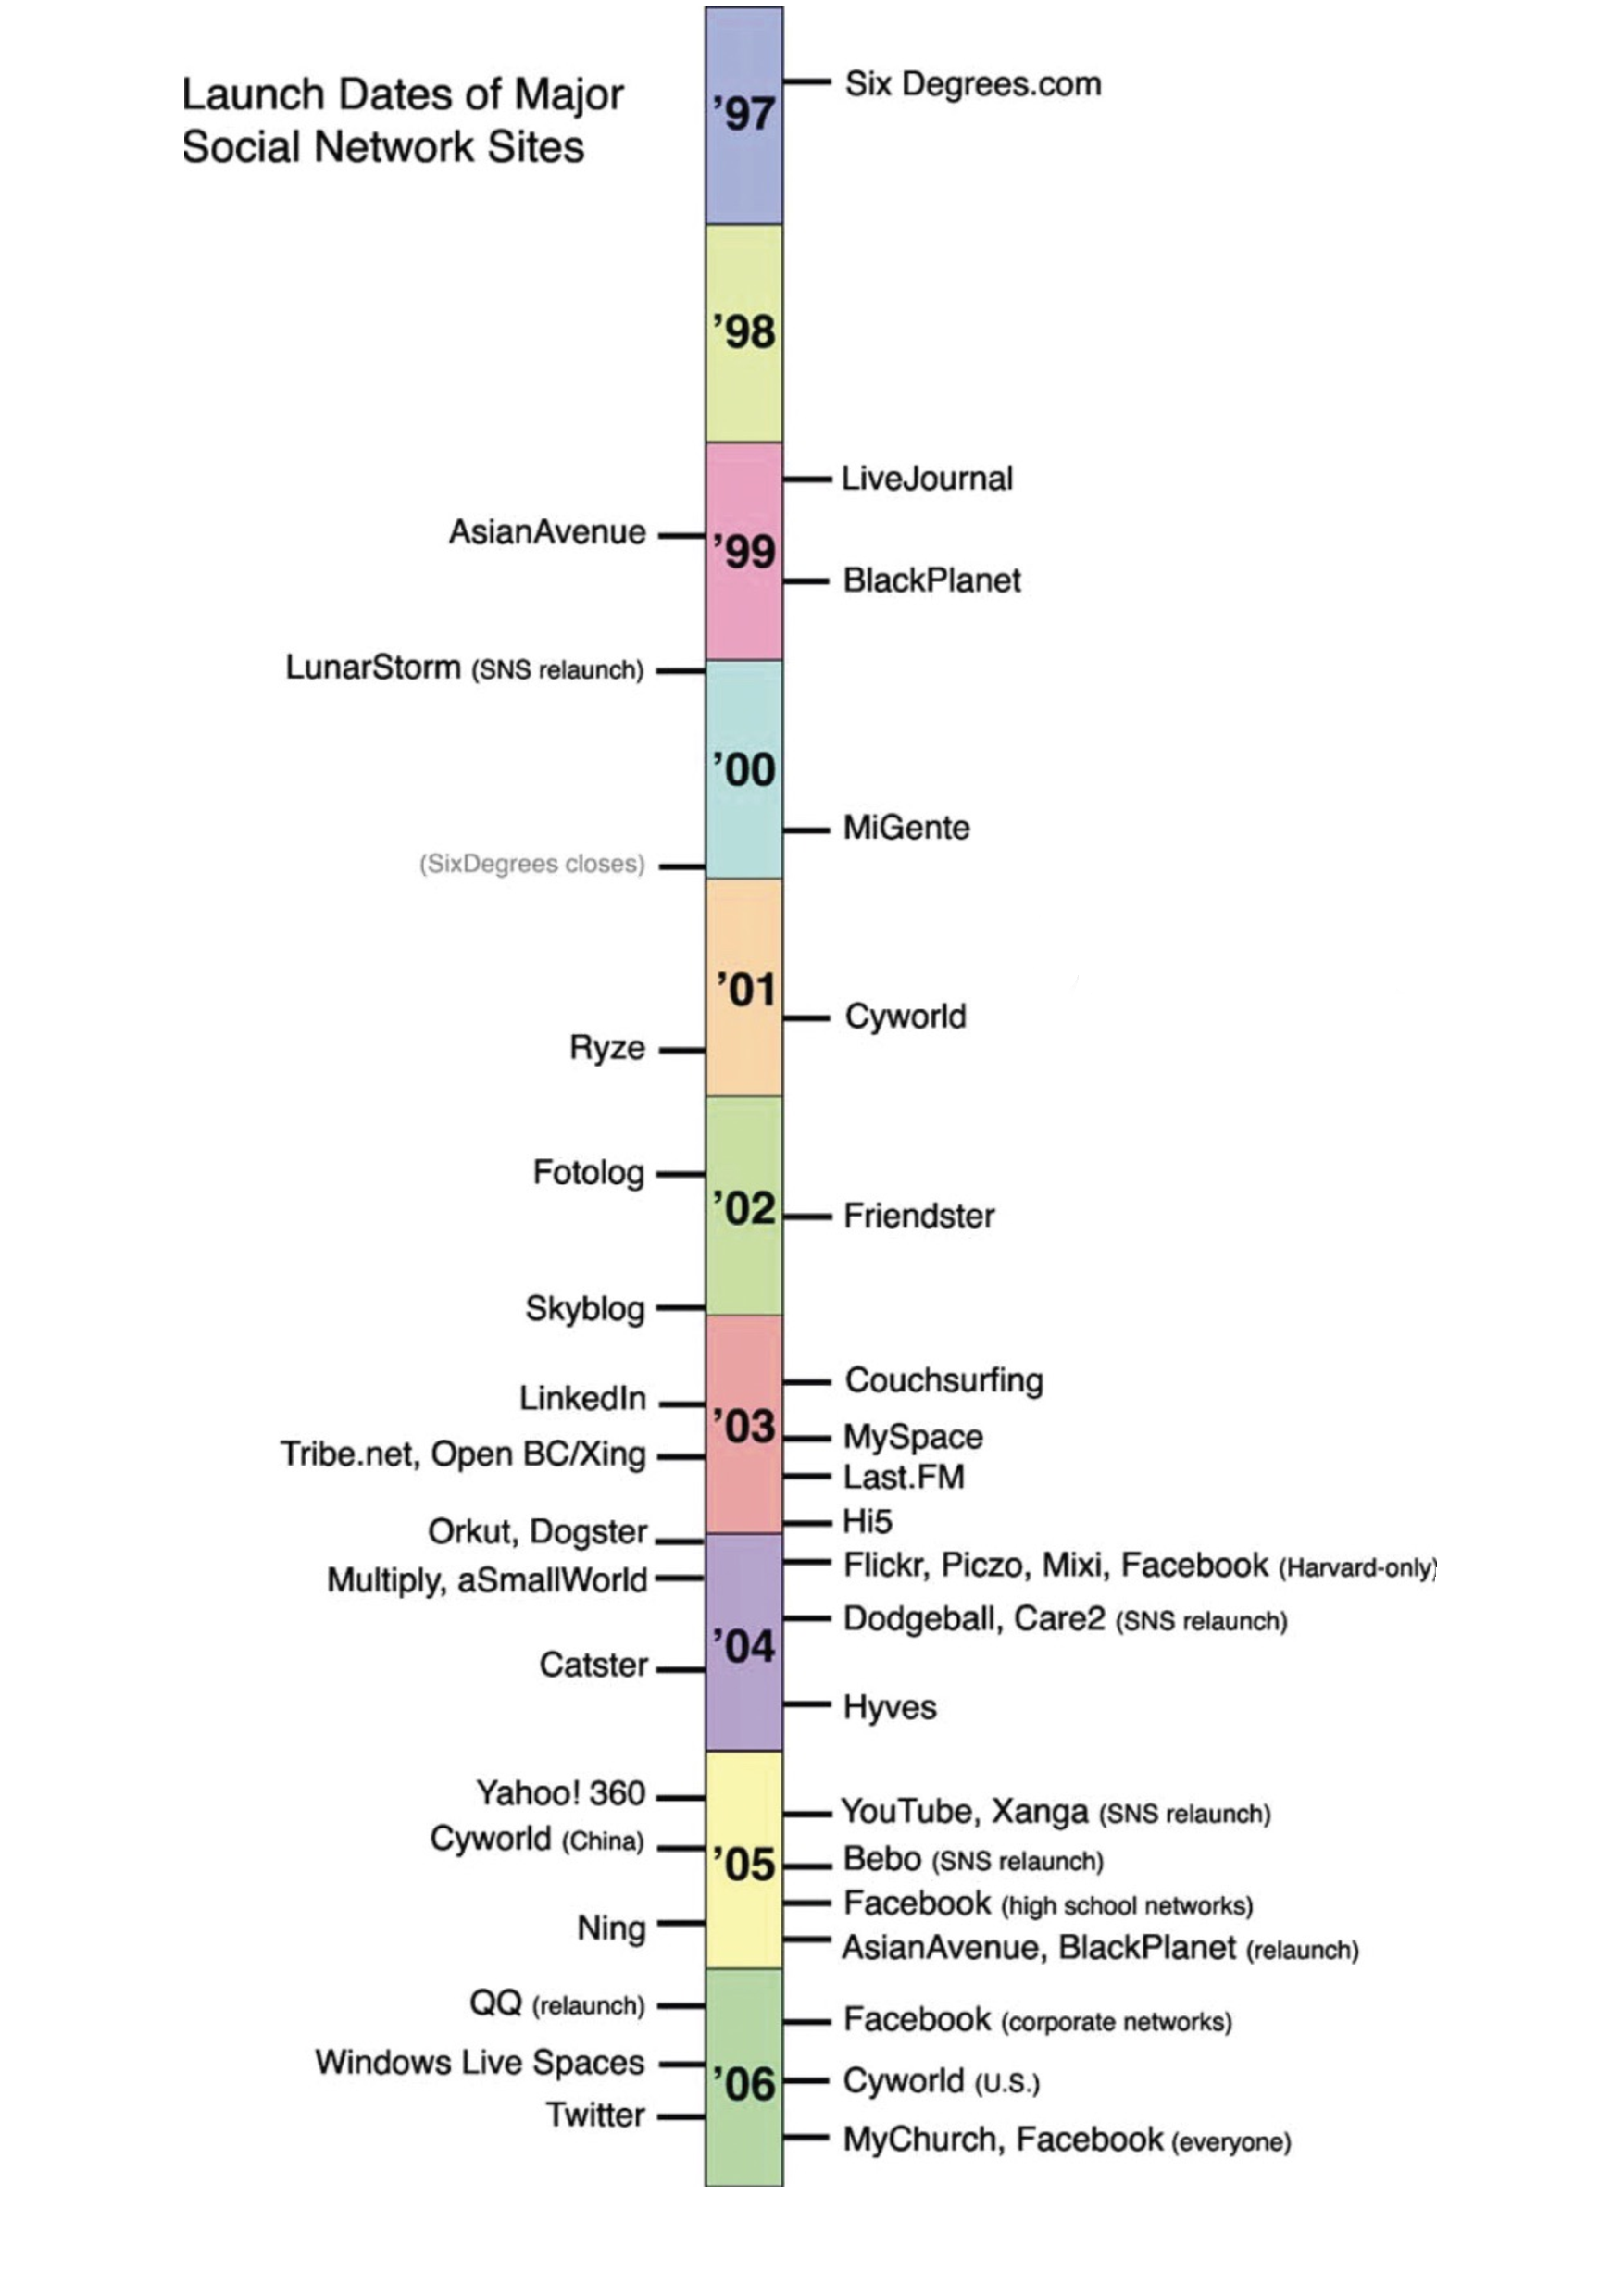
\includegraphics[width = 0.5\textwidth]{Imagenes/Vectorial/cronologiaRRSS.pdf}
	\caption{Cronología de las mayores redes sociales hasta 2006 \citep{10.1111/j.1083-6101.2007.00393.x}}
	\label{fig:cronologiaRRSS}
\end{figure}

Entre el año 1997 y el 2001, otras páginas surgieron, combinando varias funcionalidades de redes sociales como la creación de perfiles y contacto con amigos. En 2001 comenzó una nueva era para las redes sociales, con el lanzamiento de 'Ryze.com', que ayudaba a sus usuarios a incrementar sus redes de contactos empresariales.

A partir del año 2003, las redes sociales alcanzan el foco del ''mainstream'' y adquieren fama en todos los ámbitos, llegando a la población convencional. Es en esta época cuando comienzan a aparecer multitud de redes sociales, como 'LinkedIn' (evolución de 'Ryze.com'), 'MySpace' o 'Yahoo', algunas de ellas todavía activas a día de hoy.

Tras la explosión de estas redes en las cuales las personas se podían interconectar a distancia, se conviertió en un fenómeno global y fue escalando hasta el panorama que conocemos hoy en día. En los siguientes años se fundaron las redes sociales más populares que conocemos en la actualidad ('YouTube, 'Twitter', 'Facebook'...) y es en esta época también cuando se comienzan a crear redes sociales en torno a ciertos nichos, enfocadas para una pequeña parte de la población especialmente interesada en un tema en específico.

Los años 2010 sirvieron para que los gigantes de las redes sociales se afianzasen y las páginas más pequeñas cayesen por el camino. Además, al recibir tanto tráfico diario, estas empresas comenzaron a contratar multitud de ingenieros y diversificar sus negocios, entrando en sectores de diferente índole (Facebook comprando otras empresas como Instagram y potenciando su negocio de anuncios o Youtube siendo comprado por Google y ofreciendo múltiples formas de contenido, tanto vídeos largos o cortos como directos)

\section{Democratización y extensibilidad de programas informáticos}

En el mundo actual, la democratización y la extensibilidad de programas informáticos son temas cruciales. Estos conceptos no solo afectan a las personas con discapacidades, sino también a la eficiencia y la innovación en el desarrollo de software. En el caso del presente trabajo, son dos de los temas cruciales a tratar, ya que consistirá en la extensión del código ya existente en \ga, así como hacerlo más accesible para que personas con menos conocimientos técnicos también puedan emplear esta herramienta.

\subsection{Importancia de la democratización}

A día de hoy, generalmente se habla de accesibilidad para referirse a la adaptación de las nuevas tecnologías para personas con discapacidad de distintos tipos. La accesibilidad en estos casos facilita la vida de las personas, mueve la inclusividad digital y amplía el alcance de las marcas, como se explica en el estudio de \citep{kavcic2005software}. Sin embargo, en este caso, se tratará el tema de la democratización de los programas informáticos para adaptar el uso de la herramienta a perfiles no técnicos, de modo que pueda ser utilizada por gente sin conocimiento de informática y de una manera visual e intuitiva.

Promoviendo la democratización para todos los públicos, se consigue que un mayor espectro de la población pueda interactuar con este tipo de herramientas, y eventualmente puedan realizar investigaciones científicas centradas en otros ámbitos. En este caso, si algún psicólogo estuviese interesado en estudiar las relaciones sociales que ocurren entre los agentes de \ga, tendría que tener ciertos conocimientos de programación para ejecutar el programa y posiblemente no lo consiguiese, democratizando el uso de la aplicación, se puede llegar a más personas y abrir distintas líneas de investigación.

\subsection{Ejemplos de democratización}

Existen multitud de ejemplos en los que la democratización ha permitido ''viralizar'' una tecnología para que sea empleada por todos los públicos, y no solo por un sector específico, y así permitir que otros profesionales las utilicen. Algunos de estos ejemplos son los siguientes: 

\begin{itemize}
	
	\item \textbf{WordPress}: Uno de los ejemplos más conocidos es el caso de WordPress, un sistema de gestión de contenidos (CMS por sus siglas en inglés) que permite la creación de sitios web al proporcionar una plataforma accesible y fácil de usar para usuarios de todos los niveles de habilidad, desde principiantes hasta desarrolladores avanzados.
	
	\item \textbf{Unity}: Ha democratizado el desarrollo de videojuegos al ofrecer una herramienta accesible y potente para creadores de todos los niveles de habilidad, lo que permite que incluso los desarrolladores independientes produzcan juegos de alta calidad. Por lo cual, la barrera de entrada al sector del desarrollo de videojuegos es ahora mucho menor, ya que aprender esta tecnología es considerablemente más sencillo que utilizar sus predecesoras.
	
	\item \textbf{Adobe Creative Cloud}: Permite el acceso a herramientas de diseño profesional al ofrecer planes de suscripción a precios más asequibles que las licencias tradicionales. Similar al caso de Unity, los usuarios siguen necesitando cierto nivel técnico, pero las barreras de entrada al uso de las tecnologías es menor.

	
\end{itemize}

En este trabajo se pretende democratizar el uso de la investigación realizada en \ga para que pueda ser empleada por cualquier persona sin nociones de programación.

\subsection{Importancia de la extensibilidad}

La extensibilidad en los sistemas informáticos es un concepto fundamental. Consiste en la capacidad de un sistema para adaptarse y crecer mediante la incorporación de nuevas funcionalidades o características de manera sencilla y eficiente. Lo cual es esencial para el desarrollo de software, impulsado especialmente por las demandas cambiantes de los usuarios. La extensibilidad es importante tanto desde un punto de vista técnico como desde el punto de vista comercial.

Técnicamente, la extensibilidad permite que el software sea más flexible y adaptable según evolucionan los requerimientos y tecnologías. Al tener un diseño extensible, los desarrolladores pueden agregar nuevas características de manera modular, lo que facilita el mantenimiento y la escalabilidad del sistema a largo plazo.

Desde el punto de vista comercial, la extensibilidad fomenta la colaboración y la innovación al permitir que múltiples personas contribuyan al desarrollo de un sistema. Esto es especialmente relevante en proyectos de código abierto y en entornos de desarrollo colaborativo donde diferentes equipos o comunidades pueden trabajar en conjunto para mejorar un software compartido.

Según un estudio \citep{mockus2002two} sobre la evolución del software de código abierto, se encontró que la capacidad de extensibilidad era un factor crucial para el éxito y la longevidad de los proyectos, atrayendo así a nuevos colaboradores externos y manteniendo una comunidad activa de desarrollo a lo largo del tiempo.

\subsection{Ejemplos de extensibilidad}

Se ha visto que la extensibilidad es en definitiva positiva para el desarrollo del software. Por esto, existen multitud de proyectos altamente exitosos que se conciencian de producir software fácilmente extensible para mejorar la calidad del mismo. Algunos ejemplos son los siguientes:

\begin{itemize}
	
	\item \textbf{Mozilla}: El estudio mencionado anteriormente  \citep{mockus2002two} se basa específicamente en los programas Mozilla y Apache para realizar la investigación y alcanzar los resultados. Dentro de la empresa, destaca especialmente su navegador, Firefox, como ejemplo de programa extensible. Mozilla Firefox es conocido por su arquitectura extensible que permite a los usuarios instalar complementos o extensiones para personalizar y ampliar la funcionalidad del navegador, como pueden ser bloqueadores de anuncios, gestores de contraseñas o herramientas de otras índoles.
	
	\item \textbf{WordPress}: De nuevo, WordPress, además de haber creado una herramienta usable por todos los públicos, también es un claro ejemplo de extensibilidad de las funcionalidades de la aplicación. WordPress permite a los usuarios instalar temas y otros accesorios para así personalizar y extender las funcionalidades del sistema. Los temas permiten a los usuarios cambiar el diseño y la apariencia de sus sitios web, mientras que los complementos agregan nuevas características y funcionalidades, como formularios de contacto, tiendas en línea y sistemas de gestión de membresías. Según un estudio, esta extensibilidad ha sido clave para el éxito y la adopción generalizada al permitir la personalización total del contenido.
	
	\item \textbf{Visual Studio Code}: Es un editor de código fuente que también representa otro ejemplo de un software que utiliza la extensibilidad para permitir a los usuarios personalizar y ampliar el editor de código base con extensiones. Las extensiones de VS Code pueden agregar soporte para diferentes lenguajes de programación, herramientas de productividad, integración con servicios en la nube y mucho más. Además, permite el desarrollo en distintos lenguajes de progrmaación, lo que lo hace más generalista y extensible.
	
	
\end{itemize}

